
% Default to the notebook output style

    


% Inherit from the specified cell style.




    
\documentclass[11pt]{article}

    
    
    \usepackage[T1]{fontenc}
    % Nicer default font (+ math font) than Computer Modern for most use cases
    \usepackage{mathpazo}

    % Basic figure setup, for now with no caption control since it's done
    % automatically by Pandoc (which extracts ![](path) syntax from Markdown).
    \usepackage{graphicx}
    % We will generate all images so they have a width \maxwidth. This means
    % that they will get their normal width if they fit onto the page, but
    % are scaled down if they would overflow the margins.
    \makeatletter
    \def\maxwidth{\ifdim\Gin@nat@width>\linewidth\linewidth
    \else\Gin@nat@width\fi}
    \makeatother
    \let\Oldincludegraphics\includegraphics
    % Set max figure width to be 80% of text width, for now hardcoded.
    \renewcommand{\includegraphics}[1]{\Oldincludegraphics[width=.8\maxwidth]{#1}}
    % Ensure that by default, figures have no caption (until we provide a
    % proper Figure object with a Caption API and a way to capture that
    % in the conversion process - todo).
    \usepackage{caption}
    \DeclareCaptionLabelFormat{nolabel}{}
    \captionsetup{labelformat=nolabel}

    \usepackage{adjustbox} % Used to constrain images to a maximum size 
    \usepackage{xcolor} % Allow colors to be defined
    \usepackage{enumerate} % Needed for markdown enumerations to work
    \usepackage{geometry} % Used to adjust the document margins
    \usepackage{amsmath} % Equations
    \usepackage{amssymb} % Equations
    \usepackage{textcomp} % defines textquotesingle
    % Hack from http://tex.stackexchange.com/a/47451/13684:
    \AtBeginDocument{%
        \def\PYZsq{\textquotesingle}% Upright quotes in Pygmentized code
    }
    \usepackage{upquote} % Upright quotes for verbatim code
    \usepackage{eurosym} % defines \euro
    \usepackage[mathletters]{ucs} % Extended unicode (utf-8) support
    \usepackage[utf8x]{inputenc} % Allow utf-8 characters in the tex document
    \usepackage{fancyvrb} % verbatim replacement that allows latex
    \usepackage{grffile} % extends the file name processing of package graphics 
                         % to support a larger range 
    % The hyperref package gives us a pdf with properly built
    % internal navigation ('pdf bookmarks' for the table of contents,
    % internal cross-reference links, web links for URLs, etc.)
    \usepackage{hyperref}
    \usepackage{longtable} % longtable support required by pandoc >1.10
    \usepackage{booktabs}  % table support for pandoc > 1.12.2
    \usepackage[inline]{enumitem} % IRkernel/repr support (it uses the enumerate* environment)
    \usepackage[normalem]{ulem} % ulem is needed to support strikethroughs (\sout)
                                % normalem makes italics be italics, not underlines
    

    
    
    % Colors for the hyperref package
    \definecolor{urlcolor}{rgb}{0,.145,.698}
    \definecolor{linkcolor}{rgb}{.71,0.21,0.01}
    \definecolor{citecolor}{rgb}{.12,.54,.11}

    % ANSI colors
    \definecolor{ansi-black}{HTML}{3E424D}
    \definecolor{ansi-black-intense}{HTML}{282C36}
    \definecolor{ansi-red}{HTML}{E75C58}
    \definecolor{ansi-red-intense}{HTML}{B22B31}
    \definecolor{ansi-green}{HTML}{00A250}
    \definecolor{ansi-green-intense}{HTML}{007427}
    \definecolor{ansi-yellow}{HTML}{DDB62B}
    \definecolor{ansi-yellow-intense}{HTML}{B27D12}
    \definecolor{ansi-blue}{HTML}{208FFB}
    \definecolor{ansi-blue-intense}{HTML}{0065CA}
    \definecolor{ansi-magenta}{HTML}{D160C4}
    \definecolor{ansi-magenta-intense}{HTML}{A03196}
    \definecolor{ansi-cyan}{HTML}{60C6C8}
    \definecolor{ansi-cyan-intense}{HTML}{258F8F}
    \definecolor{ansi-white}{HTML}{C5C1B4}
    \definecolor{ansi-white-intense}{HTML}{A1A6B2}

    % commands and environments needed by pandoc snippets
    % extracted from the output of `pandoc -s`
    \providecommand{\tightlist}{%
      \setlength{\itemsep}{0pt}\setlength{\parskip}{0pt}}
    \DefineVerbatimEnvironment{Highlighting}{Verbatim}{commandchars=\\\{\}}
    % Add ',fontsize=\small' for more characters per line
    \newenvironment{Shaded}{}{}
    \newcommand{\KeywordTok}[1]{\textcolor[rgb]{0.00,0.44,0.13}{\textbf{{#1}}}}
    \newcommand{\DataTypeTok}[1]{\textcolor[rgb]{0.56,0.13,0.00}{{#1}}}
    \newcommand{\DecValTok}[1]{\textcolor[rgb]{0.25,0.63,0.44}{{#1}}}
    \newcommand{\BaseNTok}[1]{\textcolor[rgb]{0.25,0.63,0.44}{{#1}}}
    \newcommand{\FloatTok}[1]{\textcolor[rgb]{0.25,0.63,0.44}{{#1}}}
    \newcommand{\CharTok}[1]{\textcolor[rgb]{0.25,0.44,0.63}{{#1}}}
    \newcommand{\StringTok}[1]{\textcolor[rgb]{0.25,0.44,0.63}{{#1}}}
    \newcommand{\CommentTok}[1]{\textcolor[rgb]{0.38,0.63,0.69}{\textit{{#1}}}}
    \newcommand{\OtherTok}[1]{\textcolor[rgb]{0.00,0.44,0.13}{{#1}}}
    \newcommand{\AlertTok}[1]{\textcolor[rgb]{1.00,0.00,0.00}{\textbf{{#1}}}}
    \newcommand{\FunctionTok}[1]{\textcolor[rgb]{0.02,0.16,0.49}{{#1}}}
    \newcommand{\RegionMarkerTok}[1]{{#1}}
    \newcommand{\ErrorTok}[1]{\textcolor[rgb]{1.00,0.00,0.00}{\textbf{{#1}}}}
    \newcommand{\NormalTok}[1]{{#1}}
    
    % Additional commands for more recent versions of Pandoc
    \newcommand{\ConstantTok}[1]{\textcolor[rgb]{0.53,0.00,0.00}{{#1}}}
    \newcommand{\SpecialCharTok}[1]{\textcolor[rgb]{0.25,0.44,0.63}{{#1}}}
    \newcommand{\VerbatimStringTok}[1]{\textcolor[rgb]{0.25,0.44,0.63}{{#1}}}
    \newcommand{\SpecialStringTok}[1]{\textcolor[rgb]{0.73,0.40,0.53}{{#1}}}
    \newcommand{\ImportTok}[1]{{#1}}
    \newcommand{\DocumentationTok}[1]{\textcolor[rgb]{0.73,0.13,0.13}{\textit{{#1}}}}
    \newcommand{\AnnotationTok}[1]{\textcolor[rgb]{0.38,0.63,0.69}{\textbf{\textit{{#1}}}}}
    \newcommand{\CommentVarTok}[1]{\textcolor[rgb]{0.38,0.63,0.69}{\textbf{\textit{{#1}}}}}
    \newcommand{\VariableTok}[1]{\textcolor[rgb]{0.10,0.09,0.49}{{#1}}}
    \newcommand{\ControlFlowTok}[1]{\textcolor[rgb]{0.00,0.44,0.13}{\textbf{{#1}}}}
    \newcommand{\OperatorTok}[1]{\textcolor[rgb]{0.40,0.40,0.40}{{#1}}}
    \newcommand{\BuiltInTok}[1]{{#1}}
    \newcommand{\ExtensionTok}[1]{{#1}}
    \newcommand{\PreprocessorTok}[1]{\textcolor[rgb]{0.74,0.48,0.00}{{#1}}}
    \newcommand{\AttributeTok}[1]{\textcolor[rgb]{0.49,0.56,0.16}{{#1}}}
    \newcommand{\InformationTok}[1]{\textcolor[rgb]{0.38,0.63,0.69}{\textbf{\textit{{#1}}}}}
    \newcommand{\WarningTok}[1]{\textcolor[rgb]{0.38,0.63,0.69}{\textbf{\textit{{#1}}}}}
    
    
    % Define a nice break command that doesn't care if a line doesn't already
    % exist.
    \def\br{\hspace*{\fill} \\* }
    % Math Jax compatability definitions
    \def\gt{>}
    \def\lt{<}
    % Document parameters
    \title{Flowers Recognition-AMI\_GPU}
    
    
    

    % Pygments definitions
    
\makeatletter
\def\PY@reset{\let\PY@it=\relax \let\PY@bf=\relax%
    \let\PY@ul=\relax \let\PY@tc=\relax%
    \let\PY@bc=\relax \let\PY@ff=\relax}
\def\PY@tok#1{\csname PY@tok@#1\endcsname}
\def\PY@toks#1+{\ifx\relax#1\empty\else%
    \PY@tok{#1}\expandafter\PY@toks\fi}
\def\PY@do#1{\PY@bc{\PY@tc{\PY@ul{%
    \PY@it{\PY@bf{\PY@ff{#1}}}}}}}
\def\PY#1#2{\PY@reset\PY@toks#1+\relax+\PY@do{#2}}

\expandafter\def\csname PY@tok@w\endcsname{\def\PY@tc##1{\textcolor[rgb]{0.73,0.73,0.73}{##1}}}
\expandafter\def\csname PY@tok@c\endcsname{\let\PY@it=\textit\def\PY@tc##1{\textcolor[rgb]{0.25,0.50,0.50}{##1}}}
\expandafter\def\csname PY@tok@cp\endcsname{\def\PY@tc##1{\textcolor[rgb]{0.74,0.48,0.00}{##1}}}
\expandafter\def\csname PY@tok@k\endcsname{\let\PY@bf=\textbf\def\PY@tc##1{\textcolor[rgb]{0.00,0.50,0.00}{##1}}}
\expandafter\def\csname PY@tok@kp\endcsname{\def\PY@tc##1{\textcolor[rgb]{0.00,0.50,0.00}{##1}}}
\expandafter\def\csname PY@tok@kt\endcsname{\def\PY@tc##1{\textcolor[rgb]{0.69,0.00,0.25}{##1}}}
\expandafter\def\csname PY@tok@o\endcsname{\def\PY@tc##1{\textcolor[rgb]{0.40,0.40,0.40}{##1}}}
\expandafter\def\csname PY@tok@ow\endcsname{\let\PY@bf=\textbf\def\PY@tc##1{\textcolor[rgb]{0.67,0.13,1.00}{##1}}}
\expandafter\def\csname PY@tok@nb\endcsname{\def\PY@tc##1{\textcolor[rgb]{0.00,0.50,0.00}{##1}}}
\expandafter\def\csname PY@tok@nf\endcsname{\def\PY@tc##1{\textcolor[rgb]{0.00,0.00,1.00}{##1}}}
\expandafter\def\csname PY@tok@nc\endcsname{\let\PY@bf=\textbf\def\PY@tc##1{\textcolor[rgb]{0.00,0.00,1.00}{##1}}}
\expandafter\def\csname PY@tok@nn\endcsname{\let\PY@bf=\textbf\def\PY@tc##1{\textcolor[rgb]{0.00,0.00,1.00}{##1}}}
\expandafter\def\csname PY@tok@ne\endcsname{\let\PY@bf=\textbf\def\PY@tc##1{\textcolor[rgb]{0.82,0.25,0.23}{##1}}}
\expandafter\def\csname PY@tok@nv\endcsname{\def\PY@tc##1{\textcolor[rgb]{0.10,0.09,0.49}{##1}}}
\expandafter\def\csname PY@tok@no\endcsname{\def\PY@tc##1{\textcolor[rgb]{0.53,0.00,0.00}{##1}}}
\expandafter\def\csname PY@tok@nl\endcsname{\def\PY@tc##1{\textcolor[rgb]{0.63,0.63,0.00}{##1}}}
\expandafter\def\csname PY@tok@ni\endcsname{\let\PY@bf=\textbf\def\PY@tc##1{\textcolor[rgb]{0.60,0.60,0.60}{##1}}}
\expandafter\def\csname PY@tok@na\endcsname{\def\PY@tc##1{\textcolor[rgb]{0.49,0.56,0.16}{##1}}}
\expandafter\def\csname PY@tok@nt\endcsname{\let\PY@bf=\textbf\def\PY@tc##1{\textcolor[rgb]{0.00,0.50,0.00}{##1}}}
\expandafter\def\csname PY@tok@nd\endcsname{\def\PY@tc##1{\textcolor[rgb]{0.67,0.13,1.00}{##1}}}
\expandafter\def\csname PY@tok@s\endcsname{\def\PY@tc##1{\textcolor[rgb]{0.73,0.13,0.13}{##1}}}
\expandafter\def\csname PY@tok@sd\endcsname{\let\PY@it=\textit\def\PY@tc##1{\textcolor[rgb]{0.73,0.13,0.13}{##1}}}
\expandafter\def\csname PY@tok@si\endcsname{\let\PY@bf=\textbf\def\PY@tc##1{\textcolor[rgb]{0.73,0.40,0.53}{##1}}}
\expandafter\def\csname PY@tok@se\endcsname{\let\PY@bf=\textbf\def\PY@tc##1{\textcolor[rgb]{0.73,0.40,0.13}{##1}}}
\expandafter\def\csname PY@tok@sr\endcsname{\def\PY@tc##1{\textcolor[rgb]{0.73,0.40,0.53}{##1}}}
\expandafter\def\csname PY@tok@ss\endcsname{\def\PY@tc##1{\textcolor[rgb]{0.10,0.09,0.49}{##1}}}
\expandafter\def\csname PY@tok@sx\endcsname{\def\PY@tc##1{\textcolor[rgb]{0.00,0.50,0.00}{##1}}}
\expandafter\def\csname PY@tok@m\endcsname{\def\PY@tc##1{\textcolor[rgb]{0.40,0.40,0.40}{##1}}}
\expandafter\def\csname PY@tok@gh\endcsname{\let\PY@bf=\textbf\def\PY@tc##1{\textcolor[rgb]{0.00,0.00,0.50}{##1}}}
\expandafter\def\csname PY@tok@gu\endcsname{\let\PY@bf=\textbf\def\PY@tc##1{\textcolor[rgb]{0.50,0.00,0.50}{##1}}}
\expandafter\def\csname PY@tok@gd\endcsname{\def\PY@tc##1{\textcolor[rgb]{0.63,0.00,0.00}{##1}}}
\expandafter\def\csname PY@tok@gi\endcsname{\def\PY@tc##1{\textcolor[rgb]{0.00,0.63,0.00}{##1}}}
\expandafter\def\csname PY@tok@gr\endcsname{\def\PY@tc##1{\textcolor[rgb]{1.00,0.00,0.00}{##1}}}
\expandafter\def\csname PY@tok@ge\endcsname{\let\PY@it=\textit}
\expandafter\def\csname PY@tok@gs\endcsname{\let\PY@bf=\textbf}
\expandafter\def\csname PY@tok@gp\endcsname{\let\PY@bf=\textbf\def\PY@tc##1{\textcolor[rgb]{0.00,0.00,0.50}{##1}}}
\expandafter\def\csname PY@tok@go\endcsname{\def\PY@tc##1{\textcolor[rgb]{0.53,0.53,0.53}{##1}}}
\expandafter\def\csname PY@tok@gt\endcsname{\def\PY@tc##1{\textcolor[rgb]{0.00,0.27,0.87}{##1}}}
\expandafter\def\csname PY@tok@err\endcsname{\def\PY@bc##1{\setlength{\fboxsep}{0pt}\fcolorbox[rgb]{1.00,0.00,0.00}{1,1,1}{\strut ##1}}}
\expandafter\def\csname PY@tok@kc\endcsname{\let\PY@bf=\textbf\def\PY@tc##1{\textcolor[rgb]{0.00,0.50,0.00}{##1}}}
\expandafter\def\csname PY@tok@kd\endcsname{\let\PY@bf=\textbf\def\PY@tc##1{\textcolor[rgb]{0.00,0.50,0.00}{##1}}}
\expandafter\def\csname PY@tok@kn\endcsname{\let\PY@bf=\textbf\def\PY@tc##1{\textcolor[rgb]{0.00,0.50,0.00}{##1}}}
\expandafter\def\csname PY@tok@kr\endcsname{\let\PY@bf=\textbf\def\PY@tc##1{\textcolor[rgb]{0.00,0.50,0.00}{##1}}}
\expandafter\def\csname PY@tok@bp\endcsname{\def\PY@tc##1{\textcolor[rgb]{0.00,0.50,0.00}{##1}}}
\expandafter\def\csname PY@tok@fm\endcsname{\def\PY@tc##1{\textcolor[rgb]{0.00,0.00,1.00}{##1}}}
\expandafter\def\csname PY@tok@vc\endcsname{\def\PY@tc##1{\textcolor[rgb]{0.10,0.09,0.49}{##1}}}
\expandafter\def\csname PY@tok@vg\endcsname{\def\PY@tc##1{\textcolor[rgb]{0.10,0.09,0.49}{##1}}}
\expandafter\def\csname PY@tok@vi\endcsname{\def\PY@tc##1{\textcolor[rgb]{0.10,0.09,0.49}{##1}}}
\expandafter\def\csname PY@tok@vm\endcsname{\def\PY@tc##1{\textcolor[rgb]{0.10,0.09,0.49}{##1}}}
\expandafter\def\csname PY@tok@sa\endcsname{\def\PY@tc##1{\textcolor[rgb]{0.73,0.13,0.13}{##1}}}
\expandafter\def\csname PY@tok@sb\endcsname{\def\PY@tc##1{\textcolor[rgb]{0.73,0.13,0.13}{##1}}}
\expandafter\def\csname PY@tok@sc\endcsname{\def\PY@tc##1{\textcolor[rgb]{0.73,0.13,0.13}{##1}}}
\expandafter\def\csname PY@tok@dl\endcsname{\def\PY@tc##1{\textcolor[rgb]{0.73,0.13,0.13}{##1}}}
\expandafter\def\csname PY@tok@s2\endcsname{\def\PY@tc##1{\textcolor[rgb]{0.73,0.13,0.13}{##1}}}
\expandafter\def\csname PY@tok@sh\endcsname{\def\PY@tc##1{\textcolor[rgb]{0.73,0.13,0.13}{##1}}}
\expandafter\def\csname PY@tok@s1\endcsname{\def\PY@tc##1{\textcolor[rgb]{0.73,0.13,0.13}{##1}}}
\expandafter\def\csname PY@tok@mb\endcsname{\def\PY@tc##1{\textcolor[rgb]{0.40,0.40,0.40}{##1}}}
\expandafter\def\csname PY@tok@mf\endcsname{\def\PY@tc##1{\textcolor[rgb]{0.40,0.40,0.40}{##1}}}
\expandafter\def\csname PY@tok@mh\endcsname{\def\PY@tc##1{\textcolor[rgb]{0.40,0.40,0.40}{##1}}}
\expandafter\def\csname PY@tok@mi\endcsname{\def\PY@tc##1{\textcolor[rgb]{0.40,0.40,0.40}{##1}}}
\expandafter\def\csname PY@tok@il\endcsname{\def\PY@tc##1{\textcolor[rgb]{0.40,0.40,0.40}{##1}}}
\expandafter\def\csname PY@tok@mo\endcsname{\def\PY@tc##1{\textcolor[rgb]{0.40,0.40,0.40}{##1}}}
\expandafter\def\csname PY@tok@ch\endcsname{\let\PY@it=\textit\def\PY@tc##1{\textcolor[rgb]{0.25,0.50,0.50}{##1}}}
\expandafter\def\csname PY@tok@cm\endcsname{\let\PY@it=\textit\def\PY@tc##1{\textcolor[rgb]{0.25,0.50,0.50}{##1}}}
\expandafter\def\csname PY@tok@cpf\endcsname{\let\PY@it=\textit\def\PY@tc##1{\textcolor[rgb]{0.25,0.50,0.50}{##1}}}
\expandafter\def\csname PY@tok@c1\endcsname{\let\PY@it=\textit\def\PY@tc##1{\textcolor[rgb]{0.25,0.50,0.50}{##1}}}
\expandafter\def\csname PY@tok@cs\endcsname{\let\PY@it=\textit\def\PY@tc##1{\textcolor[rgb]{0.25,0.50,0.50}{##1}}}

\def\PYZbs{\char`\\}
\def\PYZus{\char`\_}
\def\PYZob{\char`\{}
\def\PYZcb{\char`\}}
\def\PYZca{\char`\^}
\def\PYZam{\char`\&}
\def\PYZlt{\char`\<}
\def\PYZgt{\char`\>}
\def\PYZsh{\char`\#}
\def\PYZpc{\char`\%}
\def\PYZdl{\char`\$}
\def\PYZhy{\char`\-}
\def\PYZsq{\char`\'}
\def\PYZdq{\char`\"}
\def\PYZti{\char`\~}
% for compatibility with earlier versions
\def\PYZat{@}
\def\PYZlb{[}
\def\PYZrb{]}
\makeatother


    % Exact colors from NB
    \definecolor{incolor}{rgb}{0.0, 0.0, 0.5}
    \definecolor{outcolor}{rgb}{0.545, 0.0, 0.0}



    
    % Prevent overflowing lines due to hard-to-break entities
    \sloppy 
    % Setup hyperref package
    \hypersetup{
      breaklinks=true,  % so long urls are correctly broken across lines
      colorlinks=true,
      urlcolor=urlcolor,
      linkcolor=linkcolor,
      citecolor=citecolor,
      }
    % Slightly bigger margins than the latex defaults
    
    \geometry{verbose,tmargin=1in,bmargin=1in,lmargin=1in,rmargin=1in}
    
    

    \begin{document}
    
    
    \maketitle
    
    

    
    Machine Learning Engineering nano Degree

Capstone Project - Rémi Ang

Flowers recognition

\begin{figure}
\centering
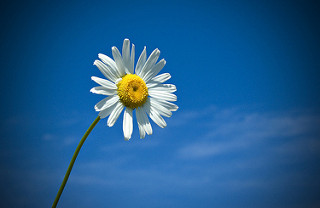
\includegraphics{./images_samples/813445367_187ecf080a_n.jpg}
\caption{Daisy}
\end{figure}

\begin{center}\rule{0.5\linewidth}{\linethickness}\end{center}

** Introduction **

This aim of this notebook is to define and train a Deep Convolutional
Network able to recognize flower species based on a picture.

The dataset is the
\href{https://www.kaggle.com/alxmamaev/flowers-recognition}{"Flowers
Recognition"} dataset from Kaggle donated by
\href{https://www.kaggle.com/alxmamaev}{Alexander Mamaev}.

The dataset contains 4362 pictures devided in 5 classes: Daisy,
Dandelion, Rose, Sunflower, Tulip

\begin{center}\rule{0.5\linewidth}{\linethickness}\end{center}

\textbf{Notebook summary:}

\begin{itemize}
\tightlist
\item
  Section \ref{step1} : Imports and print packages version
\item
  Section \ref{step2} : Scan the flowers pictures dataset
\item
  Section \ref{step3} : Visualize some pictures
\item
  Section \ref{step4} : Flowers classes distribution
\item
  Section \ref{step5} : stratified Train/test split the data and copy
  pictures in train/test folders
\item
  Section \ref{step6} : Data augmentation - create images generators
\item
  Section \ref{step7} : Convolutional Neural Network conception,
  Transfer Learning from Xception
\item
  Section \ref{step8} : train the model
\item
  Section \ref{step9} : load best weights
\item
  Section \ref{step10} : compute accuracy
\end{itemize}

     \#\# 1. imports Section \ref{top}

    \begin{Verbatim}[commandchars=\\\{\}]
{\color{incolor}In [{\color{incolor}1}]:} \PY{c+c1}{\PYZsh{} \PYZsh{} reload modules}
        \PY{c+c1}{\PYZsh{}import importlib}
        \PY{c+c1}{\PYZsh{}}
        \PY{c+c1}{\PYZsh{}import custom\PYZus{}utils}
        \PY{c+c1}{\PYZsh{}importlib.reload(custom\PYZus{}utils)}
        \PY{c+c1}{\PYZsh{}}
        \PY{c+c1}{\PYZsh{}from custom\PYZus{}utils import print\PYZus{}list, plot\PYZus{}images, flowersDistBarplot, copy\PYZus{}pictures, plotTrainingHistory, timeElapsed}
\end{Verbatim}


    \begin{Verbatim}[commandchars=\\\{\}]
{\color{incolor}In [{\color{incolor}2}]:} \PY{n+nb}{print}\PY{p}{(}\PY{l+s+s2}{\PYZdq{}}\PY{l+s+s2}{loading basic packages...}\PY{l+s+s2}{\PYZdq{}}\PY{p}{)}
        \PY{k+kn}{from} \PY{n+nn}{time} \PY{k}{import} \PY{n}{time}
        \PY{n}{start} \PY{o}{=} \PY{n}{time}\PY{p}{(}\PY{p}{)}
        
        \PY{k+kn}{import} \PY{n+nn}{sys}
        \PY{k+kn}{import} \PY{n+nn}{os}
        
        \PY{c+c1}{\PYZsh{}import glob}
        \PY{k+kn}{import} \PY{n+nn}{urllib}
        \PY{k+kn}{import} \PY{n+nn}{random}
        \PY{k+kn}{import} \PY{n+nn}{itertools}
        \PY{k+kn}{from} \PY{n+nn}{shutil} \PY{k}{import} \PY{n}{rmtree}
        
        \PY{k+kn}{from} \PY{n+nn}{tqdm} \PY{k}{import} \PY{n}{tqdm}
        
        \PY{n+nb}{print}\PY{p}{(}\PY{l+s+s2}{\PYZdq{}}\PY{l+s+s2}{loading custom utilities package...}\PY{l+s+s2}{\PYZdq{}}\PY{p}{)}
        \PY{k+kn}{from} \PY{n+nn}{custom\PYZus{}utils} \PY{k}{import} \PY{n}{print\PYZus{}list}\PY{p}{,} \PY{n}{plot\PYZus{}images}\PY{p}{,} \PY{n}{flowersDistBarplot}\PY{p}{,} \PY{n}{copy\PYZus{}pictures}\PY{p}{,} \PY{n}{plotTrainingHistory}\PY{p}{,} \PY{n}{timeElapsed}
        
        \PY{n+nb}{print}\PY{p}{(}\PY{l+s+s2}{\PYZdq{}}\PY{l+s+s2}{loading plotting packages...}\PY{l+s+s2}{\PYZdq{}}\PY{p}{)}
        \PY{k+kn}{import} \PY{n+nn}{matplotlib} \PY{k}{as} \PY{n+nn}{mlp}
        \PY{o}{\PYZpc{}}\PY{k}{matplotlib} inline  
        
        \PY{k+kn}{import} \PY{n+nn}{matplotlib}\PY{n+nn}{.}\PY{n+nn}{pyplot} \PY{k}{as} \PY{n+nn}{plt}
        \PY{c+c1}{\PYZsh{}plt.style.use(\PYZsq{}ggplot\PYZsq{})}
        
        \PY{k+kn}{import} \PY{n+nn}{seaborn} \PY{k}{as} \PY{n+nn}{sns}
        
        \PY{n+nb}{print}\PY{p}{(}\PY{l+s+s2}{\PYZdq{}}\PY{l+s+s2}{loading Numpy...}\PY{l+s+s2}{\PYZdq{}}\PY{p}{)}
        \PY{k+kn}{import} \PY{n+nn}{numpy} \PY{k}{as} \PY{n+nn}{np}
        
        \PY{n+nb}{print}\PY{p}{(}\PY{l+s+s2}{\PYZdq{}}\PY{l+s+s2}{loading Sklearn...}\PY{l+s+s2}{\PYZdq{}}\PY{p}{)}
        \PY{k+kn}{from} \PY{n+nn}{sklearn} \PY{k}{import} \PY{n}{\PYZus{}\PYZus{}version\PYZus{}\PYZus{}} \PY{k}{as} \PY{n}{sklearn\PYZus{}version}
        \PY{k+kn}{from} \PY{n+nn}{sklearn}\PY{n+nn}{.}\PY{n+nn}{datasets} \PY{k}{import} \PY{n}{load\PYZus{}files} 
        \PY{k+kn}{from} \PY{n+nn}{sklearn}\PY{n+nn}{.}\PY{n+nn}{model\PYZus{}selection} \PY{k}{import} \PY{n}{train\PYZus{}test\PYZus{}split}
        
        \PY{n+nb}{print}\PY{p}{(}\PY{l+s+s2}{\PYZdq{}}\PY{l+s+s2}{loading Keras...}\PY{l+s+s2}{\PYZdq{}}\PY{p}{)}
        \PY{c+c1}{\PYZsh{} set TensorFlow as Keras backend}
        \PY{n}{os}\PY{o}{.}\PY{n}{environ}\PY{p}{[}\PY{l+s+s1}{\PYZsq{}}\PY{l+s+s1}{KERAS\PYZus{}BACKEND}\PY{l+s+s1}{\PYZsq{}}\PY{p}{]} \PY{o}{=} \PY{l+s+s1}{\PYZsq{}}\PY{l+s+s1}{tensorflow}\PY{l+s+s1}{\PYZsq{}}
        \PY{k+kn}{from} \PY{n+nn}{keras} \PY{k}{import} \PY{n}{\PYZus{}\PYZus{}version\PYZus{}\PYZus{}} \PY{k}{as} \PY{n}{keras\PYZus{}version}
        \PY{k+kn}{from} \PY{n+nn}{keras}\PY{n+nn}{.}\PY{n+nn}{utils} \PY{k}{import} \PY{n}{np\PYZus{}utils}
        \PY{k+kn}{from} \PY{n+nn}{keras}\PY{n+nn}{.}\PY{n+nn}{preprocessing}\PY{n+nn}{.}\PY{n+nn}{image} \PY{k}{import} \PY{n}{ImageDataGenerator}
        
        \PY{c+c1}{\PYZsh{}from keras.applications.xception import Xception}
        \PY{c+c1}{\PYZsh{}import keras.applications.xception as xception }
        
        \PY{c+c1}{\PYZsh{}from keras.applications.vgg16 import VGG16}
        \PY{c+c1}{\PYZsh{}from keras.applications.resnet50 import ResNet50}
        \PY{c+c1}{\PYZsh{}from keras.applications.inception\PYZus{}v3 import InceptionV3}
        
        \PY{k+kn}{from} \PY{n+nn}{keras}\PY{n+nn}{.}\PY{n+nn}{layers} \PY{k}{import} \PY{n}{Flatten}\PY{p}{,} \PY{n}{Dense}\PY{p}{,} \PY{n}{Dropout}
        \PY{k+kn}{from} \PY{n+nn}{keras}\PY{n+nn}{.}\PY{n+nn}{models} \PY{k}{import} \PY{n}{Model}\PY{p}{,} \PY{n}{Sequential}
        \PY{k+kn}{from} \PY{n+nn}{keras}\PY{n+nn}{.}\PY{n+nn}{optimizers} \PY{k}{import} \PY{n}{Adam}
        \PY{k+kn}{from} \PY{n+nn}{keras}\PY{n+nn}{.}\PY{n+nn}{callbacks} \PY{k}{import} \PY{n}{ModelCheckpoint}  
        
        \PY{n+nb}{print}\PY{p}{(}\PY{l+s+s2}{\PYZdq{}}\PY{l+s+s2}{loading TensorFlow...}\PY{l+s+s2}{\PYZdq{}}\PY{p}{)}
        \PY{k+kn}{from} \PY{n+nn}{tensorflow} \PY{k}{import} \PY{n}{\PYZus{}\PYZus{}version\PYZus{}\PYZus{}} \PY{k}{as} \PY{n}{tf\PYZus{}version}
        
        \PY{n+nb}{print}\PY{p}{(}\PY{l+s+s2}{\PYZdq{}}\PY{l+s+s2}{loading OpenCV...}\PY{l+s+s2}{\PYZdq{}}\PY{p}{)}
        \PY{k+kn}{import} \PY{n+nn}{cv2}
        
        \PY{c+c1}{\PYZsh{} define random seed}
        \PY{n}{random\PYZus{}seed} \PY{o}{=} \PY{l+m+mi}{6}
        
        \PY{n+nb}{print}\PY{p}{(}\PY{l+s+s2}{\PYZdq{}}\PY{l+s+s2}{all imports done (time elapsed: }\PY{l+s+si}{\PYZob{}:.2f\PYZcb{}}\PY{l+s+s2}{ s)}\PY{l+s+s2}{\PYZdq{}}\PY{o}{.}\PY{n}{format}\PY{p}{(}\PY{n}{time}\PY{p}{(}\PY{p}{)} \PY{o}{\PYZhy{}} \PY{n}{start}\PY{p}{)}\PY{p}{)}
\end{Verbatim}


    \begin{Verbatim}[commandchars=\\\{\}]
loading basic packages{\ldots}
loading custom utilities package{\ldots}
loading plotting packages{\ldots}
loading Numpy{\ldots}
loading Sklearn{\ldots}
loading Keras{\ldots}

    \end{Verbatim}

    \begin{Verbatim}[commandchars=\\\{\}]
Using TensorFlow backend.
/usr/lib64/python3.4/importlib/\_bootstrap.py:321: FutureWarning: Conversion of the second argument of issubdtype from `float` to `np.floating` is deprecated. In future, it will be treated as `np.float64 == np.dtype(float).type`.
  return f(*args, **kwds)

    \end{Verbatim}

    \begin{Verbatim}[commandchars=\\\{\}]
loading TensorFlow{\ldots}
loading OpenCV{\ldots}
all imports done (time elapsed: 1.98 s)

    \end{Verbatim}

    \begin{Verbatim}[commandchars=\\\{\}]
{\color{incolor}In [{\color{incolor}3}]:} \PY{c+c1}{\PYZsh{} print packages version}
        
        \PY{n+nb}{print}\PY{p}{(}\PY{l+s+s2}{\PYZdq{}}\PY{l+s+s2}{Packages versions:}\PY{l+s+s2}{\PYZdq{}}\PY{p}{)}
        \PY{n+nb}{print}\PY{p}{(}\PY{l+s+s2}{\PYZdq{}}\PY{l+s+s2}{\PYZhy{}\PYZhy{}\PYZhy{}\PYZhy{}\PYZhy{}\PYZhy{}\PYZhy{}\PYZhy{}\PYZhy{}\PYZhy{}\PYZhy{}\PYZhy{}\PYZhy{}\PYZhy{}\PYZhy{}\PYZhy{}\PYZhy{}\PYZhy{}}\PY{l+s+s2}{\PYZdq{}}\PY{p}{)}
        \PY{n+nb}{print}\PY{p}{(}\PY{l+s+s2}{\PYZdq{}}\PY{l+s+s2}{Python: }\PY{l+s+si}{\PYZob{}\PYZcb{}}\PY{l+s+s2}{\PYZdq{}}\PY{o}{.}\PY{n}{format}\PY{p}{(}\PY{n}{sys}\PY{o}{.}\PY{n}{version}\PY{p}{)}\PY{p}{)}
        \PY{n+nb}{print}\PY{p}{(}\PY{l+s+s2}{\PYZdq{}}\PY{l+s+s2}{Matplotlib : }\PY{l+s+si}{\PYZob{}\PYZcb{}}\PY{l+s+s2}{\PYZdq{}}\PY{o}{.}\PY{n}{format}\PY{p}{(}\PY{n}{mlp}\PY{o}{.}\PY{n}{\PYZus{}\PYZus{}version\PYZus{}\PYZus{}}\PY{p}{)}\PY{p}{)}
        \PY{n+nb}{print}\PY{p}{(}\PY{l+s+s2}{\PYZdq{}}\PY{l+s+s2}{Seaborn : }\PY{l+s+si}{\PYZob{}\PYZcb{}}\PY{l+s+s2}{\PYZdq{}}\PY{o}{.}\PY{n}{format}\PY{p}{(}\PY{n}{sns}\PY{o}{.}\PY{n}{\PYZus{}\PYZus{}version\PYZus{}\PYZus{}}\PY{p}{)}\PY{p}{)}
        \PY{n+nb}{print}\PY{p}{(}\PY{l+s+s2}{\PYZdq{}}\PY{l+s+s2}{Numpy : }\PY{l+s+si}{\PYZob{}\PYZcb{}}\PY{l+s+s2}{\PYZdq{}}\PY{o}{.}\PY{n}{format}\PY{p}{(}\PY{n}{np}\PY{o}{.}\PY{n}{\PYZus{}\PYZus{}version\PYZus{}\PYZus{}}\PY{p}{)}\PY{p}{)}
        \PY{n+nb}{print}\PY{p}{(}\PY{l+s+s2}{\PYZdq{}}\PY{l+s+s2}{Scikit\PYZhy{}learn : }\PY{l+s+si}{\PYZob{}\PYZcb{}}\PY{l+s+s2}{\PYZdq{}}\PY{o}{.}\PY{n}{format}\PY{p}{(}\PY{n}{sklearn\PYZus{}version}\PY{p}{)}\PY{p}{)}
        \PY{n+nb}{print}\PY{p}{(}\PY{l+s+s2}{\PYZdq{}}\PY{l+s+s2}{Keras : }\PY{l+s+si}{\PYZob{}\PYZcb{}}\PY{l+s+s2}{\PYZdq{}}\PY{o}{.}\PY{n}{format}\PY{p}{(}\PY{n}{keras\PYZus{}version}\PY{p}{)}\PY{p}{)}
        \PY{n+nb}{print}\PY{p}{(}\PY{l+s+s2}{\PYZdq{}}\PY{l+s+s2}{Keras backend: }\PY{l+s+si}{\PYZob{}\PYZcb{}}\PY{l+s+s2}{\PYZdq{}}\PY{o}{.}\PY{n}{format}\PY{p}{(}\PY{n}{os}\PY{o}{.}\PY{n}{environ}\PY{p}{[}\PY{l+s+s1}{\PYZsq{}}\PY{l+s+s1}{KERAS\PYZus{}BACKEND}\PY{l+s+s1}{\PYZsq{}}\PY{p}{]}\PY{p}{)}\PY{p}{)}
        \PY{n+nb}{print}\PY{p}{(}\PY{l+s+s2}{\PYZdq{}}\PY{l+s+s2}{Tensor Flow : }\PY{l+s+si}{\PYZob{}\PYZcb{}}\PY{l+s+s2}{\PYZdq{}}\PY{o}{.}\PY{n}{format}\PY{p}{(}\PY{n}{tf\PYZus{}version}\PY{p}{)}\PY{p}{)}
        \PY{n+nb}{print}\PY{p}{(}\PY{l+s+s2}{\PYZdq{}}\PY{l+s+s2}{openCV : }\PY{l+s+si}{\PYZob{}\PYZcb{}}\PY{l+s+s2}{\PYZdq{}}\PY{o}{.}\PY{n}{format}\PY{p}{(}\PY{n}{cv2}\PY{o}{.}\PY{n}{\PYZus{}\PYZus{}version\PYZus{}\PYZus{}}\PY{p}{)}\PY{p}{)}
\end{Verbatim}


    \begin{Verbatim}[commandchars=\\\{\}]
Packages versions:
------------------
Python: 3.4.3 (default, Nov  2 2017, 19:19:28) 
[GCC 4.8.5 20150623 (Red Hat 4.8.5-11)]
Matplotlib : 2.2.2
Seaborn : 0.8.1
Numpy : 1.14.3
Scikit-learn : 0.19.0
Keras : 2.0.2
Keras backend: tensorflow
Tensor Flow : 1.8.0
openCV : 3.4.0

    \end{Verbatim}

     \#\# 2. Scan the flowers pictures dataset Section \ref{top}

    \begin{Verbatim}[commandchars=\\\{\}]
{\color{incolor}In [{\color{incolor}4}]:} \PY{n}{path} \PY{o}{=} \PY{l+s+s2}{\PYZdq{}}\PY{l+s+s2}{./flowers}\PY{l+s+s2}{\PYZdq{}}
        \PY{k}{if} \PY{o+ow}{not} \PY{n}{os}\PY{o}{.}\PY{n}{path}\PY{o}{.}\PY{n}{exists}\PY{p}{(}\PY{n}{path}\PY{p}{)}\PY{p}{:}
            \PY{k}{raise} \PY{n+ne}{Exception}\PY{p}{(}\PY{l+s+s2}{\PYZdq{}}\PY{l+s+s2}{The Flowers Dataset is missing!}\PY{l+s+s2}{\PYZdq{}}\PY{p}{)} 
        
        \PY{n}{blacklist\PYZus{}file} \PY{o}{=} \PY{l+s+s2}{\PYZdq{}}\PY{l+s+s2}{blacklist.txt}\PY{l+s+s2}{\PYZdq{}} \PY{c+c1}{\PYZsh{} list of files to be removed drm the dataset}
        
        \PY{c+c1}{\PYZsh{}read blacklist}
        \PY{n+nb}{print}\PY{p}{(}\PY{l+s+s2}{\PYZdq{}}\PY{l+s+se}{\PYZbs{}n}\PY{l+s+s2}{reading blacklist: }\PY{l+s+si}{\PYZob{}\PYZcb{}}\PY{l+s+s2}{...}\PY{l+s+s2}{\PYZdq{}}\PY{o}{.}\PY{n}{format}\PY{p}{(}\PY{n}{blacklist\PYZus{}file}\PY{p}{)}\PY{p}{)}
        \PY{k}{with} \PY{n+nb}{open}\PY{p}{(}\PY{n}{blacklist\PYZus{}file}\PY{p}{,} \PY{l+s+s1}{\PYZsq{}}\PY{l+s+s1}{r}\PY{l+s+s1}{\PYZsq{}}\PY{p}{)} \PY{k}{as} \PY{n}{f}\PY{p}{:}
            \PY{n}{blacklist} \PY{o}{=} \PY{n}{f}\PY{o}{.}\PY{n}{readlines}\PY{p}{(}\PY{p}{)}
        \PY{n}{blacklist} \PY{o}{=} \PY{p}{[}\PY{n}{path} \PY{o}{+} \PY{n}{s}\PY{o}{.}\PY{n}{strip}\PY{p}{(}\PY{p}{)} \PY{k}{for} \PY{n}{s} \PY{o+ow}{in} \PY{n}{blacklist}\PY{p}{]}
        \PY{n+nb}{print}\PY{p}{(}\PY{l+s+s2}{\PYZdq{}}\PY{l+s+si}{\PYZob{}\PYZcb{}}\PY{l+s+s2}{ files to discard defined in blacklist}\PY{l+s+s2}{\PYZdq{}}\PY{o}{.}\PY{n}{format}\PY{p}{(}\PY{n+nb}{len}\PY{p}{(}\PY{n}{blacklist}\PY{p}{)}\PY{p}{)}\PY{p}{)}
        
        \PY{n+nb}{print}\PY{p}{(}\PY{l+s+s2}{\PYZdq{}}\PY{l+s+se}{\PYZbs{}n}\PY{l+s+s2}{Collecting files from data folder : }\PY{l+s+si}{\PYZob{}\PYZcb{}}\PY{l+s+s2}{\PYZdq{}}\PY{o}{.}\PY{n}{format}\PY{p}{(}\PY{n}{path}\PY{p}{)}\PY{p}{)}
        \PY{n}{data} \PY{o}{=} \PY{n}{load\PYZus{}files}\PY{p}{(}\PY{n}{path}\PY{p}{,} \PY{n}{load\PYZus{}content}\PY{o}{=}\PY{k+kc}{False}\PY{p}{)}
        \PY{n}{all\PYZus{}flowers\PYZus{}files} \PY{o}{=} \PY{n}{np}\PY{o}{.}\PY{n}{array}\PY{p}{(}\PY{p}{[}\PY{n}{s}\PY{o}{.}\PY{n}{replace}\PY{p}{(}\PY{l+s+s1}{\PYZsq{}}\PY{l+s+se}{\PYZbs{}\PYZbs{}}\PY{l+s+s1}{\PYZsq{}}\PY{p}{,} \PY{l+s+s1}{\PYZsq{}}\PY{l+s+s1}{/}\PY{l+s+s1}{\PYZsq{}}\PY{p}{)} \PY{k}{for} \PY{n}{s} \PY{o+ow}{in} \PY{n}{data}\PY{p}{[}\PY{l+s+s2}{\PYZdq{}}\PY{l+s+s2}{filenames}\PY{l+s+s2}{\PYZdq{}}\PY{p}{]}\PY{p}{]}\PY{p}{)}
        \PY{n+nb}{print}\PY{p}{(}\PY{l+s+s2}{\PYZdq{}}\PY{l+s+si}{\PYZob{}\PYZcb{}}\PY{l+s+s2}{ flower pictures found}\PY{l+s+s2}{\PYZdq{}}\PY{o}{.}\PY{n}{format}\PY{p}{(}\PY{n}{all\PYZus{}flowers\PYZus{}files}\PY{o}{.}\PY{n}{shape}\PY{p}{[}\PY{l+m+mi}{0}\PY{p}{]}\PY{p}{)}\PY{p}{)}
        
        \PY{c+c1}{\PYZsh{} identify blacklist indexes}
        \PY{n}{isvalid\PYZus{}file} \PY{o}{=} \PY{p}{[}\PY{k+kc}{True} \PY{k}{if} \PY{n}{f} \PY{o+ow}{not} \PY{o+ow}{in} \PY{n}{blacklist} \PY{k}{else} \PY{k+kc}{False} \PY{k}{for} \PY{n}{f} \PY{o+ow}{in} \PY{n}{all\PYZus{}flowers\PYZus{}files}\PY{p}{]}
        \PY{n}{flowers\PYZus{}files} \PY{o}{=} \PY{n}{all\PYZus{}flowers\PYZus{}files}\PY{p}{[}\PY{n}{isvalid\PYZus{}file}\PY{p}{]}
        \PY{n+nb}{print}\PY{p}{(}\PY{l+s+s2}{\PYZdq{}}\PY{l+s+si}{\PYZob{}\PYZcb{}}\PY{l+s+s2}{ flower pictures kept after black list filtering}\PY{l+s+s2}{\PYZdq{}}\PY{o}{.}\PY{n}{format}\PY{p}{(}\PY{n}{flowers\PYZus{}files}\PY{o}{.}\PY{n}{shape}\PY{p}{[}\PY{l+m+mi}{0}\PY{p}{]}\PY{p}{)}\PY{p}{)}
        
        \PY{c+c1}{\PYZsh{} flowers\PYZus{}targets = np\PYZus{}utils.to\PYZus{}categorical(data[\PYZdq{}target\PYZdq{}],5)}
        \PY{n}{flowers\PYZus{}targets} \PY{o}{=} \PY{n}{data}\PY{p}{[}\PY{l+s+s2}{\PYZdq{}}\PY{l+s+s2}{target}\PY{l+s+s2}{\PYZdq{}}\PY{p}{]}\PY{p}{[}\PY{n}{isvalid\PYZus{}file}\PY{p}{]}
        \PY{n}{flowers\PYZus{}target\PYZus{}names} \PY{o}{=} \PY{n}{data}\PY{p}{[}\PY{l+s+s2}{\PYZdq{}}\PY{l+s+s2}{target\PYZus{}names}\PY{l+s+s2}{\PYZdq{}}\PY{p}{]}
        
        \PY{n+nb}{print}\PY{p}{(}\PY{p}{)}
        \PY{n}{print\PYZus{}list}\PY{p}{(}\PY{n}{flowers\PYZus{}target\PYZus{}names}\PY{p}{,} \PY{l+s+s1}{\PYZsq{}}\PY{l+s+s1}{types of flower found}\PY{l+s+s1}{\PYZsq{}}\PY{p}{)}
\end{Verbatim}


    \begin{Verbatim}[commandchars=\\\{\}]

reading blacklist: blacklist.txt{\ldots}
1059 files to discard defined in blacklist

Collecting files from data folder : ./flowers
4326 flower pictures found
3268 flower pictures kept after black list filtering

5 types of flower found:
	o daisy
	o dandelion
	o rose
	o sunflower
	o tulip

    \end{Verbatim}

     \#\# 3. Visualize some pictures Section \ref{top}

    \begin{Verbatim}[commandchars=\\\{\}]
{\color{incolor}In [{\color{incolor}5}]:} \PY{c+c1}{\PYZsh{}np.random.seed(0)}
        \PY{n}{n\PYZus{}samples} \PY{o}{=} \PY{l+m+mi}{15}
        \PY{n}{sample\PYZus{}idx} \PY{o}{=} \PY{n}{np}\PY{o}{.}\PY{n}{random}\PY{o}{.}\PY{n}{choice}\PY{p}{(}\PY{n+nb}{list}\PY{p}{(}\PY{n+nb}{range}\PY{p}{(}\PY{n}{flowers\PYZus{}files}\PY{o}{.}\PY{n}{shape}\PY{p}{[}\PY{l+m+mi}{0}\PY{p}{]}\PY{p}{)}\PY{p}{)}\PY{p}{,} \PY{n}{n\PYZus{}samples}\PY{p}{)}
        \PY{n}{sample\PYZus{}files} \PY{o}{=} \PY{n}{flowers\PYZus{}files}\PY{p}{[}\PY{n}{sample\PYZus{}idx}\PY{p}{]}
        \PY{n}{sample\PYZus{}titles} \PY{o}{=} \PY{p}{[}\PY{n}{flowers\PYZus{}target\PYZus{}names}\PY{p}{[}\PY{n}{i}\PY{p}{]} \PY{k}{for} \PY{n}{i} \PY{o+ow}{in} \PY{n}{flowers\PYZus{}targets}\PY{p}{[}\PY{n}{sample\PYZus{}idx}\PY{p}{]}\PY{p}{]}
        
        \PY{n}{plot\PYZus{}images}\PY{p}{(}\PY{n}{sample\PYZus{}files}\PY{p}{,} \PY{n}{sample\PYZus{}titles}\PY{p}{)}
\end{Verbatim}


    \begin{center}
    \adjustimage{max size={0.9\linewidth}{0.9\paperheight}}{output_8_0.png}
    \end{center}
    { \hspace*{\fill} \\}
    
    ** Note: ** the flower pictures are of various sizes, angle of view,
light conditions. We can also observe that some pictures have been
artistically post-processed, adding colour filters altering the original
colour of the flower. In some case the flower is not the main subject of
the picture, as such we often have on the picture non-flower subjects
such as insects, babies, wine bottle, etc.

The Dandelion flower appear in 2 states: the yellow-orange flower and
the whithe spherical seeds head "blowball" form.

    \subsubsection{black listed picture
samples}\label{black-listed-picture-samples}

    \begin{Verbatim}[commandchars=\\\{\}]
{\color{incolor}In [{\color{incolor}6}]:} \PY{c+c1}{\PYZsh{}np.random.seed(4)}
        \PY{n}{n\PYZus{}samples} \PY{o}{=} \PY{l+m+mi}{15}
        \PY{n}{sample\PYZus{}idx} \PY{o}{=} \PY{n}{np}\PY{o}{.}\PY{n}{random}\PY{o}{.}\PY{n}{choice}\PY{p}{(}\PY{n+nb}{list}\PY{p}{(}\PY{n+nb}{range}\PY{p}{(}\PY{n+nb}{len}\PY{p}{(}\PY{n}{blacklist}\PY{p}{)}\PY{p}{)}\PY{p}{)}\PY{p}{,} \PY{n}{n\PYZus{}samples}\PY{p}{)}
        \PY{n}{sample\PYZus{}files} \PY{o}{=} \PY{n}{np}\PY{o}{.}\PY{n}{array}\PY{p}{(}\PY{n}{blacklist}\PY{p}{)}\PY{p}{[}\PY{n}{sample\PYZus{}idx}\PY{p}{]}
        
        \PY{n}{sample\PYZus{}titles} \PY{o}{=} \PY{p}{[}\PY{p}{]}\PY{p}{;}
        \PY{k}{for} \PY{n}{sample\PYZus{}file} \PY{o+ow}{in} \PY{n}{sample\PYZus{}files}\PY{p}{:}
            \PY{n}{idx} \PY{o}{=} \PY{n}{np}\PY{o}{.}\PY{n}{where}\PY{p}{(}\PY{n}{all\PYZus{}flowers\PYZus{}files} \PY{o}{==} \PY{n}{sample\PYZus{}file}\PY{p}{)}
            \PY{n}{sample\PYZus{}titles}\PY{o}{.}\PY{n}{append}\PY{p}{(}\PY{n}{flowers\PYZus{}target\PYZus{}names}\PY{p}{[}\PY{n}{data}\PY{p}{[}\PY{l+s+s2}{\PYZdq{}}\PY{l+s+s2}{target}\PY{l+s+s2}{\PYZdq{}}\PY{p}{]}\PY{p}{[}\PY{n}{idx}\PY{p}{]}\PY{p}{[}\PY{l+m+mi}{0}\PY{p}{]}\PY{p}{]}\PY{p}{)}
            
        
        \PY{n+nb}{print}\PY{p}{(}\PY{l+s+s2}{\PYZdq{}}\PY{l+s+s2}{\PYZdq{}}\PY{p}{)}
        \PY{n}{plot\PYZus{}images}\PY{p}{(}\PY{n}{sample\PYZus{}files}\PY{p}{,} \PY{n}{sample\PYZus{}titles}\PY{p}{)}
\end{Verbatim}


    \begin{Verbatim}[commandchars=\\\{\}]


    \end{Verbatim}

    \begin{center}
    \adjustimage{max size={0.9\linewidth}{0.9\paperheight}}{output_11_1.png}
    \end{center}
    { \hspace*{\fill} \\}
    
     \#\# 4. Flowers Classes distribution Section \ref{top}

    \begin{Verbatim}[commandchars=\\\{\}]
{\color{incolor}In [{\color{incolor}7}]:} \PY{n}{flowersDistBarplot}\PY{p}{(}\PY{n}{flowers\PYZus{}targets}\PY{p}{,} \PY{n}{flowers\PYZus{}target\PYZus{}names}\PY{p}{,} \PY{l+s+s2}{\PYZdq{}}\PY{l+s+s2}{Flowers types distribution}\PY{l+s+s2}{\PYZdq{}}\PY{p}{)}
\end{Verbatim}


    \begin{center}
    \adjustimage{max size={0.9\linewidth}{0.9\paperheight}}{output_13_0.png}
    \end{center}
    { \hspace*{\fill} \\}
    
    ** Note : ** classes distribution is slightly unbalanced.

    \href{https://keras.io/applications/}{keras applications reference page}

     \#\# 5. stratified Train/Valid/Test split of the dataset
Section \ref{top}

** Note ** : stratified split is required to preserve a uniform
distirbution of each class in both train and tests split

    \begin{Verbatim}[commandchars=\\\{\}]
{\color{incolor}In [{\color{incolor}8}]:} \PY{c+c1}{\PYZsh{}np.random.seed(random\PYZus{}seed)}
        
        \PY{n}{test\PYZus{}size} \PY{o}{=} \PY{o}{.}\PY{l+m+mi}{1}
        
        \PY{n+nb}{print}\PY{p}{(}\PY{l+s+s2}{\PYZdq{}}\PY{l+s+s2}{Splitting train+valid/test flower files (split ratio: }\PY{l+s+si}{\PYZob{}\PYZcb{}}\PY{l+s+s2}{ / }\PY{l+s+si}{\PYZob{}\PYZcb{}}\PY{l+s+s2}{ }\PY{l+s+s2}{\PYZpc{}}\PY{l+s+s2}{)...}\PY{l+s+s2}{\PYZdq{}}\PY{o}{.}\PY{n}{format}\PY{p}{(}\PY{p}{(}\PY{l+m+mi}{1}\PY{o}{\PYZhy{}}\PY{n}{test\PYZus{}size}\PY{p}{)} \PY{o}{*} \PY{l+m+mi}{100}\PY{p}{,} \PY{n}{test\PYZus{}size} \PY{o}{*} \PY{l+m+mi}{100}\PY{p}{)}\PY{p}{)}
        \PY{n}{flowers\PYZus{}files\PYZus{}train\PYZus{}valid}\PY{p}{,} \PY{n}{flowers\PYZus{}files\PYZus{}test}\PY{p}{,} \PY{n}{flowers\PYZus{}targets\PYZus{}train\PYZus{}valid}\PY{p}{,} \PY{n}{flowers\PYZus{}targets\PYZus{}test} \PY{o}{=} \PY{n}{train\PYZus{}test\PYZus{}split}\PY{p}{(}
            \PY{n}{flowers\PYZus{}files}\PY{p}{,} \PY{n}{flowers\PYZus{}targets}\PY{p}{,} 
            \PY{n}{test\PYZus{}size} \PY{o}{=} \PY{n}{test\PYZus{}size}\PY{p}{,} 
            \PY{n}{stratify}\PY{o}{=}\PY{n}{flowers\PYZus{}targets}\PY{p}{,}
            \PY{n}{random\PYZus{}state}\PY{o}{=}\PY{n}{random\PYZus{}seed}\PY{p}{)}
        
        
        \PY{n}{valid\PYZus{}size} \PY{o}{=} \PY{o}{.}\PY{l+m+mi}{2}
        \PY{n+nb}{print}\PY{p}{(}\PY{l+s+s2}{\PYZdq{}}\PY{l+s+s2}{Splitting train/valid flower files (split ratio: }\PY{l+s+si}{\PYZob{}\PYZcb{}}\PY{l+s+s2}{ / }\PY{l+s+si}{\PYZob{}\PYZcb{}}\PY{l+s+s2}{ }\PY{l+s+s2}{\PYZpc{}}\PY{l+s+s2}{)...}\PY{l+s+s2}{\PYZdq{}}\PY{o}{.}\PY{n}{format}\PY{p}{(}\PY{p}{(}\PY{l+m+mi}{1}\PY{o}{\PYZhy{}}\PY{n}{valid\PYZus{}size}\PY{p}{)} \PY{o}{*} \PY{l+m+mi}{100}\PY{p}{,} \PY{n}{valid\PYZus{}size} \PY{o}{*} \PY{l+m+mi}{100}\PY{p}{)}\PY{p}{)}
        \PY{n}{flowers\PYZus{}files\PYZus{}train}\PY{p}{,} \PY{n}{flowers\PYZus{}files\PYZus{}valid}\PY{p}{,} \PY{n}{flowers\PYZus{}targets\PYZus{}train}\PY{p}{,} \PY{n}{flowers\PYZus{}targets\PYZus{}valid} \PY{o}{=} \PY{n}{train\PYZus{}test\PYZus{}split}\PY{p}{(}
            \PY{n}{flowers\PYZus{}files\PYZus{}train\PYZus{}valid}\PY{p}{,} \PY{n}{flowers\PYZus{}targets\PYZus{}train\PYZus{}valid}\PY{p}{,} 
            \PY{n}{test\PYZus{}size} \PY{o}{=} \PY{n}{valid\PYZus{}size}\PY{p}{,} 
            \PY{n}{stratify}\PY{o}{=}\PY{n}{flowers\PYZus{}targets\PYZus{}train\PYZus{}valid}\PY{p}{,}
            \PY{n}{random\PYZus{}state}\PY{o}{=}\PY{n}{random\PYZus{}seed}\PY{p}{)}
        
        \PY{n+nb}{print}\PY{p}{(}\PY{l+s+s2}{\PYZdq{}}\PY{l+s+si}{\PYZob{}\PYZcb{}}\PY{l+s+s2}{ training flowers files.}\PY{l+s+s2}{\PYZdq{}}\PY{o}{.}\PY{n}{format}\PY{p}{(}\PY{n}{flowers\PYZus{}files\PYZus{}train}\PY{o}{.}\PY{n}{shape}\PY{p}{[}\PY{l+m+mi}{0}\PY{p}{]}\PY{p}{)}\PY{p}{)}
        \PY{n+nb}{print}\PY{p}{(}\PY{l+s+s2}{\PYZdq{}}\PY{l+s+si}{\PYZob{}\PYZcb{}}\PY{l+s+s2}{ validation flowers files.}\PY{l+s+s2}{\PYZdq{}}\PY{o}{.}\PY{n}{format}\PY{p}{(}\PY{n}{flowers\PYZus{}files\PYZus{}valid}\PY{o}{.}\PY{n}{shape}\PY{p}{[}\PY{l+m+mi}{0}\PY{p}{]}\PY{p}{)}\PY{p}{)}
        \PY{n+nb}{print}\PY{p}{(}\PY{l+s+s2}{\PYZdq{}}\PY{l+s+si}{\PYZob{}\PYZcb{}}\PY{l+s+s2}{ testing flowers files.}\PY{l+s+s2}{\PYZdq{}}\PY{o}{.}\PY{n}{format}\PY{p}{(}\PY{n}{flowers\PYZus{}files\PYZus{}test}\PY{o}{.}\PY{n}{shape}\PY{p}{[}\PY{l+m+mi}{0}\PY{p}{]}\PY{p}{)}\PY{p}{)}
\end{Verbatim}


    \begin{Verbatim}[commandchars=\\\{\}]
Splitting train+valid/test flower files (split ratio: 90.0 / 10.0 \%){\ldots}
Splitting train/valid flower files (split ratio: 80.0 / 20.0 \%){\ldots}
2352 training flowers files.
589 validation flowers files.
327 testing flowers files.

    \end{Verbatim}

    \begin{Verbatim}[commandchars=\\\{\}]
{\color{incolor}In [{\color{incolor}9}]:} \PY{n}{flowersDistBarplot}\PY{p}{(}\PY{p}{[}\PY{n}{flowers\PYZus{}targets\PYZus{}train}\PY{p}{,}\PY{n}{flowers\PYZus{}targets\PYZus{}valid}\PY{p}{,}\PY{n}{flowers\PYZus{}targets\PYZus{}test}\PY{p}{]}\PY{p}{,}
                           \PY{n}{flowers\PYZus{}target\PYZus{}names}\PY{p}{,} 
                           \PY{p}{[}\PY{l+s+s2}{\PYZdq{}}\PY{l+s+s2}{Training set}\PY{l+s+s2}{\PYZdq{}}\PY{p}{,}  \PY{l+s+s2}{\PYZdq{}}\PY{l+s+s2}{Validation set}\PY{l+s+s2}{\PYZdq{}}\PY{p}{,} \PY{l+s+s2}{\PYZdq{}}\PY{l+s+s2}{Testing set}\PY{l+s+s2}{\PYZdq{}}\PY{p}{]}\PY{p}{)}
\end{Verbatim}


    \begin{center}
    \adjustimage{max size={0.9\linewidth}{0.9\paperheight}}{output_18_0.png}
    \end{center}
    { \hspace*{\fill} \\}
    
    \subsection{5. 2 Load the datasets in memory, transform targets to
categorical}\label{load-the-datasets-in-memory-transform-targets-to-categorical}

    \begin{Verbatim}[commandchars=\\\{\}]
{\color{incolor}In [{\color{incolor}10}]:} \PY{k}{def} \PY{n+nf}{loadimg}\PY{p}{(}\PY{n}{path}\PY{p}{)}\PY{p}{:}
             \PY{l+s+sd}{\PYZdq{}\PYZdq{}\PYZdq{}}
         \PY{l+s+sd}{    load and resize an image}
         \PY{l+s+sd}{    return a (299, 299, 3) array}
         \PY{l+s+sd}{    \PYZdq{}\PYZdq{}\PYZdq{}}
             \PY{n}{img} \PY{o}{=} \PY{n}{cv2}\PY{o}{.}\PY{n}{imread}\PY{p}{(}\PY{n}{path}\PY{p}{)}
             \PY{n}{img\PYZus{}r} \PY{o}{=} \PY{n}{cv2}\PY{o}{.}\PY{n}{resize}\PY{p}{(}\PY{n}{img}\PY{p}{,} \PY{p}{(}\PY{l+m+mi}{299}\PY{p}{,} \PY{l+m+mi}{299}\PY{p}{)}\PY{p}{)}
             \PY{k}{return} \PY{n}{img\PYZus{}r}
\end{Verbatim}


    \begin{Verbatim}[commandchars=\\\{\}]
{\color{incolor}In [{\color{incolor}11}]:} \PY{n}{x\PYZus{}train} \PY{o}{=} \PY{n}{np}\PY{o}{.}\PY{n}{array}\PY{p}{(}\PY{p}{[}\PY{n}{loadimg}\PY{p}{(}\PY{n}{f}\PY{p}{)} \PY{k}{for} \PY{n}{f} \PY{o+ow}{in} \PY{n}{tqdm}\PY{p}{(}\PY{n}{flowers\PYZus{}files\PYZus{}train}\PY{p}{)}\PY{p}{]}\PY{p}{)}\PY{o}{.}\PY{n}{reshape}\PY{p}{(}\PY{o}{\PYZhy{}}\PY{l+m+mi}{1}\PY{p}{,} \PY{l+m+mi}{299}\PY{p}{,} \PY{l+m+mi}{299}\PY{p}{,} \PY{l+m+mi}{3}\PY{p}{)}
         \PY{n}{y\PYZus{}train} \PY{o}{=}  \PY{n}{np\PYZus{}utils}\PY{o}{.}\PY{n}{to\PYZus{}categorical}\PY{p}{(}\PY{n}{flowers\PYZus{}targets\PYZus{}train}\PY{p}{)}
         \PY{n+nb}{print}\PY{p}{(}\PY{l+s+s2}{\PYZdq{}}\PY{l+s+s2}{training set shape : }\PY{l+s+si}{\PYZob{}\PYZcb{}}\PY{l+s+s2}{\PYZdq{}}\PY{o}{.}\PY{n}{format}\PY{p}{(}\PY{n}{x\PYZus{}train}\PY{o}{.}\PY{n}{shape}\PY{p}{)}\PY{p}{)}
\end{Verbatim}


    \begin{Verbatim}[commandchars=\\\{\}]
100\%|██████████| 2352/2352 [00:05<00:00, 417.10it/s]

    \end{Verbatim}

    \begin{Verbatim}[commandchars=\\\{\}]
training set shape : (2352, 299, 299, 3)

    \end{Verbatim}

    \begin{Verbatim}[commandchars=\\\{\}]
{\color{incolor}In [{\color{incolor}12}]:} \PY{n}{x\PYZus{}valid} \PY{o}{=} \PY{n}{np}\PY{o}{.}\PY{n}{array}\PY{p}{(}\PY{p}{[}\PY{n}{loadimg}\PY{p}{(}\PY{n}{f}\PY{p}{)} \PY{k}{for} \PY{n}{f} \PY{o+ow}{in} \PY{n}{tqdm}\PY{p}{(}\PY{n}{flowers\PYZus{}files\PYZus{}valid}\PY{p}{)}\PY{p}{]}\PY{p}{)}\PY{o}{.}\PY{n}{reshape}\PY{p}{(}\PY{o}{\PYZhy{}}\PY{l+m+mi}{1}\PY{p}{,} \PY{l+m+mi}{299}\PY{p}{,} \PY{l+m+mi}{299}\PY{p}{,} \PY{l+m+mi}{3}\PY{p}{)}
         \PY{n}{y\PYZus{}valid} \PY{o}{=}  \PY{n}{np\PYZus{}utils}\PY{o}{.}\PY{n}{to\PYZus{}categorical}\PY{p}{(}\PY{n}{flowers\PYZus{}targets\PYZus{}valid}\PY{p}{)}
         \PY{n+nb}{print}\PY{p}{(}\PY{l+s+s2}{\PYZdq{}}\PY{l+s+s2}{training set shape : }\PY{l+s+si}{\PYZob{}\PYZcb{}}\PY{l+s+s2}{\PYZdq{}}\PY{o}{.}\PY{n}{format}\PY{p}{(}\PY{n}{x\PYZus{}train}\PY{o}{.}\PY{n}{shape}\PY{p}{)}\PY{p}{)}
\end{Verbatim}


    \begin{Verbatim}[commandchars=\\\{\}]
100\%|██████████| 589/589 [00:01<00:00, 408.60it/s]

    \end{Verbatim}

    \begin{Verbatim}[commandchars=\\\{\}]
training set shape : (2352, 299, 299, 3)

    \end{Verbatim}

    \begin{Verbatim}[commandchars=\\\{\}]
{\color{incolor}In [{\color{incolor}13}]:} \PY{n}{x\PYZus{}test} \PY{o}{=} \PY{n}{np}\PY{o}{.}\PY{n}{array}\PY{p}{(}\PY{p}{[}\PY{n}{loadimg}\PY{p}{(}\PY{n}{f}\PY{p}{)} \PY{k}{for} \PY{n}{f} \PY{o+ow}{in} \PY{n}{tqdm}\PY{p}{(}\PY{n}{flowers\PYZus{}files\PYZus{}test}\PY{p}{)}\PY{p}{]}\PY{p}{)}\PY{o}{.}\PY{n}{reshape}\PY{p}{(}\PY{o}{\PYZhy{}}\PY{l+m+mi}{1}\PY{p}{,} \PY{l+m+mi}{299}\PY{p}{,} \PY{l+m+mi}{299}\PY{p}{,} \PY{l+m+mi}{3}\PY{p}{)}
         \PY{n}{y\PYZus{}test} \PY{o}{=}  \PY{n}{np\PYZus{}utils}\PY{o}{.}\PY{n}{to\PYZus{}categorical}\PY{p}{(}\PY{n}{flowers\PYZus{}targets\PYZus{}test}\PY{p}{)}
         \PY{n+nb}{print}\PY{p}{(}\PY{l+s+s2}{\PYZdq{}}\PY{l+s+s2}{testing set shape : }\PY{l+s+si}{\PYZob{}\PYZcb{}}\PY{l+s+s2}{\PYZdq{}}\PY{o}{.}\PY{n}{format}\PY{p}{(}\PY{n}{x\PYZus{}test}\PY{o}{.}\PY{n}{shape}\PY{p}{)}\PY{p}{)}
\end{Verbatim}


    \begin{Verbatim}[commandchars=\\\{\}]
100\%|██████████| 327/327 [00:00<00:00, 426.14it/s]

    \end{Verbatim}

    \begin{Verbatim}[commandchars=\\\{\}]
testing set shape : (327, 299, 299, 3)

    \end{Verbatim}

     \#\# 6. Data augmentation - Create image generators Section \ref{top}

    \begin{Verbatim}[commandchars=\\\{\}]
{\color{incolor}In [{\color{incolor}14}]:} \PY{c+c1}{\PYZsh{}batch\PYZus{}size = 32 \PYZsh{} default: 32}
         
         \PY{c+c1}{\PYZsh{} training data generator \PYZhy{} scaling and data augmentation}
         \PY{n+nb}{print}\PY{p}{(}\PY{l+s+s2}{\PYZdq{}}\PY{l+s+s2}{Initializing training data generator...}\PY{l+s+s2}{\PYZdq{}}\PY{p}{)}
         \PY{n}{train\PYZus{}datagen} \PY{o}{=} \PY{n}{ImageDataGenerator}\PY{p}{(}
                 \PY{n}{rescale}\PY{o}{=}\PY{l+m+mf}{1.}\PY{o}{/}\PY{l+m+mi}{255}\PY{p}{,}
                 \PY{n}{shear\PYZus{}range}\PY{o}{=}\PY{l+m+mf}{0.2}\PY{p}{,}
                 \PY{n}{zoom\PYZus{}range}\PY{o}{=}\PY{l+m+mf}{0.2}\PY{p}{,}
                 \PY{n}{horizontal\PYZus{}flip}\PY{o}{=}\PY{k+kc}{True}\PY{p}{)}
         
         \PY{n}{train\PYZus{}datagen}\PY{o}{.}\PY{n}{fit}\PY{p}{(}\PY{n}{x\PYZus{}train}\PY{p}{)}
         \PY{c+c1}{\PYZsh{} train\PYZus{}generator = train\PYZus{}datagen.flow\PYZus{}from\PYZus{}directory(}
         \PY{c+c1}{\PYZsh{}         os.path.join(\PYZsq{}.\PYZsq{}, data\PYZus{}root, \PYZsq{}train\PYZsq{}),  }
         \PY{c+c1}{\PYZsh{}         target\PYZus{}size=(150, 150),  \PYZsh{} all images will be resized to 150x150}
         \PY{c+c1}{\PYZsh{}         batch\PYZus{}size=batch\PYZus{}size,}
         \PY{c+c1}{\PYZsh{}         class\PYZus{}mode=\PYZsq{}categorical\PYZsq{})}
         
         \PY{c+c1}{\PYZsh{} validation data generator \PYZhy{} scaling and data augmentation}
         \PY{n+nb}{print}\PY{p}{(}\PY{l+s+s2}{\PYZdq{}}\PY{l+s+s2}{Initializing validation data generator...}\PY{l+s+s2}{\PYZdq{}}\PY{p}{)}
         \PY{n}{valid\PYZus{}datagen} \PY{o}{=} \PY{n}{ImageDataGenerator}\PY{p}{(}
                 \PY{n}{rescale}\PY{o}{=}\PY{l+m+mf}{1.}\PY{o}{/}\PY{l+m+mi}{255}\PY{p}{,}
                 \PY{n}{shear\PYZus{}range}\PY{o}{=}\PY{l+m+mf}{0.2}\PY{p}{,}
                 \PY{n}{zoom\PYZus{}range}\PY{o}{=}\PY{l+m+mf}{0.2}\PY{p}{,}
                 \PY{n}{horizontal\PYZus{}flip}\PY{o}{=}\PY{k+kc}{True}\PY{p}{)}
         
         \PY{n}{valid\PYZus{}datagen}\PY{o}{.}\PY{n}{fit}\PY{p}{(}\PY{n}{x\PYZus{}valid}\PY{p}{)}
         
         \PY{c+c1}{\PYZsh{} test data generator \PYZhy{} scaling only}
         \PY{c+c1}{\PYZsh{} print(\PYZdq{}Initializing testing data generator...\PYZdq{})}
         \PY{c+c1}{\PYZsh{} test\PYZus{}datagen = ImageDataGenerator(rescale=1./255)}
         \PY{c+c1}{\PYZsh{} test\PYZus{}datagen.fit(x\PYZus{}test)}
         
         \PY{c+c1}{\PYZsh{} test\PYZus{}generator = test\PYZus{}datagen.flow\PYZus{}from\PYZus{}directory(}
         \PY{c+c1}{\PYZsh{}        os.path.join(\PYZsq{}.\PYZsq{}, data\PYZus{}root, \PYZsq{}test\PYZsq{}),  }
         \PY{c+c1}{\PYZsh{}         target\PYZus{}size=(150,150),}
         \PY{c+c1}{\PYZsh{}         batch\PYZus{}size=batch\PYZus{}size,}
         \PY{c+c1}{\PYZsh{}         class\PYZus{}mode=\PYZsq{}categorical\PYZsq{})}
\end{Verbatim}


    \begin{Verbatim}[commandchars=\\\{\}]
Initializing training data generator{\ldots}
Initializing validation data generator{\ldots}
Initializing testing data generator{\ldots}

    \end{Verbatim}

    \begin{Verbatim}[commandchars=\\\{\}]
{\color{incolor}In [{\color{incolor}15}]:} \PY{c+c1}{\PYZsh{} visualize augmented images}
         
         \PY{n}{n\PYZus{}img} \PY{o}{=} \PY{l+m+mi}{20}
         \PY{n}{max\PYZus{}img\PYZus{}per\PYZus{}row} \PY{o}{=} \PY{l+m+mi}{5}
         
         \PY{n}{n\PYZus{}rows} \PY{o}{=} \PY{n}{np}\PY{o}{.}\PY{n}{ceil}\PY{p}{(}\PY{l+m+mf}{1.}\PY{o}{*}\PY{n}{n\PYZus{}img} \PY{o}{/} \PY{n}{max\PYZus{}img\PYZus{}per\PYZus{}row}\PY{p}{)}
         
         \PY{n}{fig} \PY{o}{=} \PY{n}{plt}\PY{o}{.}\PY{n}{figure}\PY{p}{(}\PY{n}{figsize}\PY{o}{=}\PY{p}{(}\PY{l+m+mi}{20}\PY{p}{,}\PY{n}{n\PYZus{}rows}\PY{o}{*}\PY{l+m+mi}{5}\PY{p}{)}\PY{p}{)}
         \PY{k}{for} \PY{n}{x\PYZus{}batch} \PY{o+ow}{in} \PY{n}{train\PYZus{}datagen}\PY{o}{.}\PY{n}{flow}\PY{p}{(}\PY{n}{x\PYZus{}train}\PY{p}{,} \PY{n}{batch\PYZus{}size}\PY{o}{=}\PY{n}{n\PYZus{}img}\PY{p}{)}\PY{p}{:}
             \PY{k}{for} \PY{n}{i} \PY{o+ow}{in} \PY{n+nb}{range}\PY{p}{(}\PY{l+m+mi}{0}\PY{p}{,} \PY{n}{n\PYZus{}img}\PY{p}{)}\PY{p}{:}
                 \PY{n}{ax} \PY{o}{=} \PY{n}{fig}\PY{o}{.}\PY{n}{add\PYZus{}subplot}\PY{p}{(}\PY{n}{n\PYZus{}rows}\PY{p}{,} \PY{n}{max\PYZus{}img\PYZus{}per\PYZus{}row}\PY{p}{,} \PY{n}{i}\PY{o}{+}\PY{l+m+mi}{1}\PY{p}{)}
                 \PY{n}{ax}\PY{o}{.}\PY{n}{imshow}\PY{p}{(}\PY{n}{x\PYZus{}batch}\PY{p}{[}\PY{n}{i}\PY{p}{]}\PY{p}{)}
             \PY{n}{fig}\PY{o}{.}\PY{n}{suptitle}\PY{p}{(}\PY{l+s+s1}{\PYZsq{}}\PY{l+s+s1}{Augmented Images}\PY{l+s+s1}{\PYZsq{}}\PY{p}{,} \PY{n}{fontsize}\PY{o}{=}\PY{l+m+mi}{20}\PY{p}{)}
             \PY{n}{plt}\PY{o}{.}\PY{n}{show}\PY{p}{(}\PY{p}{)}
             \PY{k}{break}\PY{p}{;}
\end{Verbatim}


    \begin{center}
    \adjustimage{max size={0.9\linewidth}{0.9\paperheight}}{output_26_0.png}
    \end{center}
    { \hspace*{\fill} \\}
    
     \#\# 7. Convolutional Neural Network conception, Transfer Learning from
Xception Section \ref{top}

\href{https://www.kaggle.com/aakashnain/flowers-are-mesmerizing}{reference:
"flowers are mesmerizing", \emph{aakashnain}}

    \href{https://i.imgur.com/tA2qDIQ.jpg}{Xception}

\paragraph{VGG16 architecture}\label{vgg16-architecture}

\begin{figure}
\centering
\includegraphics{https://qph.ec.quoracdn.net/main-qimg-ba81c87204be1a5d11d64a464bca39eb}
\caption{VGG16}
\end{figure}

    \begin{Verbatim}[commandchars=\\\{\}]
{\color{incolor}In [{\color{incolor}16}]:} \PY{c+c1}{\PYZsh{} load the model (download the weights if necessary)}
         \PY{c+c1}{\PYZsh{} include\PYZus{}top : whether to include the 3 fully\PYZhy{}connected layers at the top of the network}
         
         \PY{c+c1}{\PYZsh{}from keras.applications.xception import Xception}
         \PY{c+c1}{\PYZsh{}import keras.applications.xception as xception }
         
         \PY{c+c1}{\PYZsh{}from keras.applications.vgg16 import VGG16}
         \PY{c+c1}{\PYZsh{}from keras.applications.resnet50 import ResNet50}
         \PY{c+c1}{\PYZsh{}from keras.applications.inception\PYZus{}v3 import InceptionV3}
         
         \PY{n}{base\PYZus{}model\PYZus{}name} \PY{o}{=} \PY{l+s+s1}{\PYZsq{}}\PY{l+s+s1}{VGG16}\PY{l+s+s1}{\PYZsq{}}    \PY{c+c1}{\PYZsh{} size: 99MB Top\PYZhy{}5 Accuracy: 0.929}
         \PY{c+c1}{\PYZsh{}base\PYZus{}model\PYZus{}name = \PYZsq{}ResNet50\PYZsq{}    \PYZsh{} size: 99MB Top\PYZhy{}5 Accuracy: 0.929}
         \PY{c+c1}{\PYZsh{}base\PYZus{}model\PYZus{}name = \PYZsq{}InceptionV3\PYZsq{} \PYZsh{} size: 92MB Top\PYZhy{}5 Accuracy: 0.944}
         \PY{c+c1}{\PYZsh{}base\PYZus{}model\PYZus{}name = \PYZsq{}Xception\PYZsq{}    \PYZsh{} size: 88MB Top\PYZhy{}5 Accuracy: 0.945}
         
         \PY{k}{if} \PY{n}{base\PYZus{}model\PYZus{}name} \PY{o}{==} \PY{l+s+s1}{\PYZsq{}}\PY{l+s+s1}{Xception}\PY{l+s+s1}{\PYZsq{}}\PY{p}{:}
             \PY{k+kn}{from} \PY{n+nn}{keras}\PY{n+nn}{.}\PY{n+nn}{applications}\PY{n+nn}{.}\PY{n+nn}{xception} \PY{k}{import} \PY{n}{Xception}
             \PY{n}{base\PYZus{}model} \PY{o}{=} \PY{n}{Xception}\PY{p}{(}\PY{n}{weights}\PY{o}{=}\PY{l+s+s1}{\PYZsq{}}\PY{l+s+s1}{imagenet}\PY{l+s+s1}{\PYZsq{}}\PY{p}{,} \PY{n}{include\PYZus{}top}\PY{o}{=}\PY{k+kc}{False}\PY{p}{,} \PY{n}{input\PYZus{}shape}\PY{o}{=}\PY{p}{(}\PY{l+m+mi}{299}\PY{p}{,}\PY{l+m+mi}{299}\PY{p}{,}\PY{l+m+mi}{3}\PY{p}{)}\PY{p}{)}
         \PY{k}{elif} \PY{n}{base\PYZus{}model\PYZus{}name} \PY{o}{==} \PY{l+s+s1}{\PYZsq{}}\PY{l+s+s1}{ResNet50}\PY{l+s+s1}{\PYZsq{}}\PY{p}{:}
             \PY{k+kn}{from} \PY{n+nn}{keras}\PY{n+nn}{.}\PY{n+nn}{applications}\PY{n+nn}{.}\PY{n+nn}{resnet50} \PY{k}{import} \PY{n}{ResNet50}
             \PY{n}{base\PYZus{}model} \PY{o}{=} \PY{n}{ResNet50}\PY{p}{(}\PY{n}{weights}\PY{o}{=}\PY{l+s+s1}{\PYZsq{}}\PY{l+s+s1}{imagenet}\PY{l+s+s1}{\PYZsq{}}\PY{p}{,} \PY{n}{include\PYZus{}top}\PY{o}{=}\PY{k+kc}{False}\PY{p}{,} \PY{n}{input\PYZus{}shape}\PY{o}{=}\PY{p}{(}\PY{l+m+mi}{299}\PY{p}{,}\PY{l+m+mi}{299}\PY{p}{,}\PY{l+m+mi}{3}\PY{p}{)}\PY{p}{)}   
         \PY{k}{elif} \PY{n}{base\PYZus{}model\PYZus{}name} \PY{o}{==} \PY{l+s+s1}{\PYZsq{}}\PY{l+s+s1}{InceptionV3}\PY{l+s+s1}{\PYZsq{}}\PY{p}{:}
             \PY{k+kn}{from} \PY{n+nn}{keras}\PY{n+nn}{.}\PY{n+nn}{applications}\PY{n+nn}{.}\PY{n+nn}{inception\PYZus{}v3} \PY{k}{import} \PY{n}{InceptionV3}
             \PY{n}{base\PYZus{}model} \PY{o}{=} \PY{n}{InceptionV3}\PY{p}{(}\PY{n}{weights}\PY{o}{=}\PY{l+s+s1}{\PYZsq{}}\PY{l+s+s1}{imagenet}\PY{l+s+s1}{\PYZsq{}}\PY{p}{,} \PY{n}{include\PYZus{}top}\PY{o}{=}\PY{k+kc}{False}\PY{p}{,} \PY{n}{input\PYZus{}shape}\PY{o}{=}\PY{p}{(}\PY{l+m+mi}{299}\PY{p}{,}\PY{l+m+mi}{299}\PY{p}{,}\PY{l+m+mi}{3}\PY{p}{)}\PY{p}{)}
         \PY{k}{elif} \PY{n}{base\PYZus{}model\PYZus{}name} \PY{o}{==} \PY{l+s+s1}{\PYZsq{}}\PY{l+s+s1}{VGG16}\PY{l+s+s1}{\PYZsq{}}\PY{p}{:}
             \PY{k+kn}{from} \PY{n+nn}{keras}\PY{n+nn}{.}\PY{n+nn}{applications}\PY{n+nn}{.}\PY{n+nn}{vgg16} \PY{k}{import} \PY{n}{VGG16}
             \PY{n}{base\PYZus{}model} \PY{o}{=} \PY{n}{VGG16}\PY{p}{(}\PY{n}{weights}\PY{o}{=}\PY{l+s+s1}{\PYZsq{}}\PY{l+s+s1}{imagenet}\PY{l+s+s1}{\PYZsq{}}\PY{p}{,} \PY{n}{include\PYZus{}top}\PY{o}{=}\PY{k+kc}{False}\PY{p}{,} \PY{n}{input\PYZus{}shape}\PY{o}{=}\PY{p}{(}\PY{l+m+mi}{299}\PY{p}{,}\PY{l+m+mi}{299}\PY{p}{,}\PY{l+m+mi}{3}\PY{p}{)}\PY{p}{)}  
         \PY{k}{elif} \PY{n}{base\PYZus{}model\PYZus{}name} \PY{o}{==} \PY{l+s+s1}{\PYZsq{}}\PY{l+s+s1}{VGG19}\PY{l+s+s1}{\PYZsq{}}\PY{p}{:}
             \PY{k+kn}{from} \PY{n+nn}{keras}\PY{n+nn}{.}\PY{n+nn}{applications}\PY{n+nn}{.}\PY{n+nn}{vgg19} \PY{k}{import} \PY{n}{VGG19}
             \PY{n}{base\PYZus{}model} \PY{o}{=} \PY{n}{VGG19}\PY{p}{(}\PY{n}{weights}\PY{o}{=}\PY{l+s+s1}{\PYZsq{}}\PY{l+s+s1}{imagenet}\PY{l+s+s1}{\PYZsq{}}\PY{p}{,} \PY{n}{include\PYZus{}top}\PY{o}{=}\PY{k+kc}{False}\PY{p}{,} \PY{n}{input\PYZus{}shape}\PY{o}{=}\PY{p}{(}\PY{l+m+mi}{299}\PY{p}{,}\PY{l+m+mi}{299}\PY{p}{,}\PY{l+m+mi}{3}\PY{p}{)}\PY{p}{)}     
                 
\end{Verbatim}


    \begin{Verbatim}[commandchars=\\\{\}]
{\color{incolor}In [{\color{incolor}17}]:} \PY{c+c1}{\PYZsh{} freeze the layers of the base model}
         \PY{k}{for} \PY{n}{layer} \PY{o+ow}{in} \PY{n}{base\PYZus{}model}\PY{o}{.}\PY{n}{layers}\PY{p}{:}
             \PY{n}{layer}\PY{o}{.}\PY{n}{trainable} \PY{o}{=} \PY{k+kc}{False}   
             
         \PY{c+c1}{\PYZsh{} new layers:}
         \PY{c+c1}{\PYZsh{} \PYZhy{}\PYZhy{}\PYZhy{}\PYZhy{}\PYZhy{}\PYZhy{}\PYZhy{}\PYZhy{}\PYZhy{}\PYZhy{}\PYZhy{}}
         
         \PY{n}{x} \PY{o}{=} \PY{n}{Flatten}\PY{p}{(}\PY{p}{)}\PY{p}{(}\PY{n}{base\PYZus{}model}\PY{o}{.}\PY{n}{output}\PY{p}{)}
         \PY{n}{x} \PY{o}{=} \PY{n}{Dense}\PY{p}{(}\PY{l+m+mi}{500}\PY{p}{,} \PY{n}{activation}\PY{o}{=}\PY{l+s+s1}{\PYZsq{}}\PY{l+s+s1}{relu}\PY{l+s+s1}{\PYZsq{}}\PY{p}{,} \PY{n}{name}\PY{o}{=}\PY{l+s+s1}{\PYZsq{}}\PY{l+s+s1}{fc1}\PY{l+s+s1}{\PYZsq{}}\PY{p}{)}\PY{p}{(}\PY{n}{x}\PY{p}{)}
         \PY{n}{x} \PY{o}{=} \PY{n}{Dropout}\PY{p}{(}\PY{l+m+mf}{0.3}\PY{p}{)}\PY{p}{(}\PY{n}{x}\PY{p}{)}
         \PY{n}{x} \PY{o}{=} \PY{n}{Dense}\PY{p}{(}\PY{l+m+mi}{5}\PY{p}{,} \PY{n}{activation}\PY{o}{=}\PY{l+s+s1}{\PYZsq{}}\PY{l+s+s1}{softmax}\PY{l+s+s1}{\PYZsq{}}\PY{p}{,} \PY{n}{name}\PY{o}{=}\PY{l+s+s1}{\PYZsq{}}\PY{l+s+s1}{fc2}\PY{l+s+s1}{\PYZsq{}}\PY{p}{)}\PY{p}{(}\PY{n}{x}\PY{p}{)}
         
         \PY{c+c1}{\PYZsh{} Model class API, take tensor in input and tensor in output}
         \PY{n}{model} \PY{o}{=} \PY{n}{Model}\PY{p}{(}\PY{n}{inputs}\PY{o}{=}\PY{n}{base\PYZus{}model}\PY{o}{.}\PY{n}{input}\PY{p}{,} \PY{n}{outputs}\PY{o}{=}\PY{n}{x}\PY{p}{)}
         
         \PY{c+c1}{\PYZsh{} Adam optimizer attributes:}
         \PY{c+c1}{\PYZsh{} \PYZhy{}\PYZhy{}\PYZhy{}\PYZhy{}\PYZhy{}\PYZhy{}\PYZhy{}\PYZhy{}\PYZhy{}\PYZhy{}\PYZhy{}\PYZhy{}\PYZhy{}\PYZhy{}\PYZhy{}\PYZhy{}\PYZhy{}\PYZhy{}\PYZhy{}\PYZhy{}\PYZhy{}\PYZhy{}\PYZhy{}\PYZhy{}\PYZhy{}\PYZhy{}}
         \PY{c+c1}{\PYZsh{} lr: float \PYZgt{}= 0. Learning rate.}
         \PY{c+c1}{\PYZsh{} beta\PYZus{}1: float, 0 \PYZlt{} beta \PYZlt{} 1. Generally close to 1.}
         \PY{c+c1}{\PYZsh{} beta\PYZus{}2: float, 0 \PYZlt{} beta \PYZlt{} 1. Generally close to 1.}
         \PY{c+c1}{\PYZsh{} epsilon: float \PYZgt{}= 0. Fuzz factor. If None, defaults to K.epsilon().}
         \PY{c+c1}{\PYZsh{} decay: float \PYZgt{}= 0. Learning rate decay over each update.}
         \PY{c+c1}{\PYZsh{} amsgrad: boolean. Whether to apply the AMSGrad variant of this algorithm from the paper \PYZdq{}On the Convergence of Adam and Beyond\PYZdq{}.}
         
         \PY{n}{opt} \PY{o}{=} \PY{n}{Adam}\PY{p}{(}\PY{n}{lr} \PY{o}{=} \PY{l+m+mf}{1e\PYZhy{}3}\PY{p}{,} \PY{n}{decay}\PY{o}{=}\PY{l+m+mf}{1e\PYZhy{}6}\PY{p}{)}
         \PY{c+c1}{\PYZsh{}opt = Adam(lr = 1e\PYZhy{}3)}
         
         \PY{n}{model}\PY{o}{.}\PY{n}{compile}\PY{p}{(}\PY{n}{loss} \PY{o}{=} \PY{l+s+s1}{\PYZsq{}}\PY{l+s+s1}{categorical\PYZus{}crossentropy}\PY{l+s+s1}{\PYZsq{}}\PY{p}{,} \PY{n}{optimizer}\PY{o}{=}\PY{n}{opt}\PY{p}{,} \PY{n}{metrics}\PY{o}{=}\PY{p}{[}\PY{l+s+s1}{\PYZsq{}}\PY{l+s+s1}{accuracy}\PY{l+s+s1}{\PYZsq{}}\PY{p}{]}\PY{p}{)}
         
         \PY{n}{model}\PY{o}{.}\PY{n}{summary}\PY{p}{(}\PY{p}{)}
\end{Verbatim}


    \begin{Verbatim}[commandchars=\\\{\}]
WARNING:tensorflow:From /usr/local/lib64/python3.4/site-packages/keras/backend/tensorflow\_backend.py:1062: calling reduce\_prod (from tensorflow.python.ops.math\_ops) with keep\_dims is deprecated and will be removed in a future version.
Instructions for updating:
keep\_dims is deprecated, use keepdims instead
WARNING:tensorflow:From /usr/local/lib64/python3.4/site-packages/keras/backend/tensorflow\_backend.py:2548: calling reduce\_sum (from tensorflow.python.ops.math\_ops) with keep\_dims is deprecated and will be removed in a future version.
Instructions for updating:
keep\_dims is deprecated, use keepdims instead
WARNING:tensorflow:From /usr/local/lib64/python3.4/site-packages/keras/backend/tensorflow\_backend.py:1123: calling reduce\_mean (from tensorflow.python.ops.math\_ops) with keep\_dims is deprecated and will be removed in a future version.
Instructions for updating:
keep\_dims is deprecated, use keepdims instead
\_\_\_\_\_\_\_\_\_\_\_\_\_\_\_\_\_\_\_\_\_\_\_\_\_\_\_\_\_\_\_\_\_\_\_\_\_\_\_\_\_\_\_\_\_\_\_\_\_\_\_\_\_\_\_\_\_\_\_\_\_\_\_\_\_
Layer (type)                 Output Shape              Param \#   
=================================================================
input\_1 (InputLayer)         (None, 299, 299, 3)       0         
\_\_\_\_\_\_\_\_\_\_\_\_\_\_\_\_\_\_\_\_\_\_\_\_\_\_\_\_\_\_\_\_\_\_\_\_\_\_\_\_\_\_\_\_\_\_\_\_\_\_\_\_\_\_\_\_\_\_\_\_\_\_\_\_\_
block1\_conv1 (Conv2D)        (None, 299, 299, 64)      1792      
\_\_\_\_\_\_\_\_\_\_\_\_\_\_\_\_\_\_\_\_\_\_\_\_\_\_\_\_\_\_\_\_\_\_\_\_\_\_\_\_\_\_\_\_\_\_\_\_\_\_\_\_\_\_\_\_\_\_\_\_\_\_\_\_\_
block1\_conv2 (Conv2D)        (None, 299, 299, 64)      36928     
\_\_\_\_\_\_\_\_\_\_\_\_\_\_\_\_\_\_\_\_\_\_\_\_\_\_\_\_\_\_\_\_\_\_\_\_\_\_\_\_\_\_\_\_\_\_\_\_\_\_\_\_\_\_\_\_\_\_\_\_\_\_\_\_\_
block1\_pool (MaxPooling2D)   (None, 149, 149, 64)      0         
\_\_\_\_\_\_\_\_\_\_\_\_\_\_\_\_\_\_\_\_\_\_\_\_\_\_\_\_\_\_\_\_\_\_\_\_\_\_\_\_\_\_\_\_\_\_\_\_\_\_\_\_\_\_\_\_\_\_\_\_\_\_\_\_\_
block2\_conv1 (Conv2D)        (None, 149, 149, 128)     73856     
\_\_\_\_\_\_\_\_\_\_\_\_\_\_\_\_\_\_\_\_\_\_\_\_\_\_\_\_\_\_\_\_\_\_\_\_\_\_\_\_\_\_\_\_\_\_\_\_\_\_\_\_\_\_\_\_\_\_\_\_\_\_\_\_\_
block2\_conv2 (Conv2D)        (None, 149, 149, 128)     147584    
\_\_\_\_\_\_\_\_\_\_\_\_\_\_\_\_\_\_\_\_\_\_\_\_\_\_\_\_\_\_\_\_\_\_\_\_\_\_\_\_\_\_\_\_\_\_\_\_\_\_\_\_\_\_\_\_\_\_\_\_\_\_\_\_\_
block2\_pool (MaxPooling2D)   (None, 74, 74, 128)       0         
\_\_\_\_\_\_\_\_\_\_\_\_\_\_\_\_\_\_\_\_\_\_\_\_\_\_\_\_\_\_\_\_\_\_\_\_\_\_\_\_\_\_\_\_\_\_\_\_\_\_\_\_\_\_\_\_\_\_\_\_\_\_\_\_\_
block3\_conv1 (Conv2D)        (None, 74, 74, 256)       295168    
\_\_\_\_\_\_\_\_\_\_\_\_\_\_\_\_\_\_\_\_\_\_\_\_\_\_\_\_\_\_\_\_\_\_\_\_\_\_\_\_\_\_\_\_\_\_\_\_\_\_\_\_\_\_\_\_\_\_\_\_\_\_\_\_\_
block3\_conv2 (Conv2D)        (None, 74, 74, 256)       590080    
\_\_\_\_\_\_\_\_\_\_\_\_\_\_\_\_\_\_\_\_\_\_\_\_\_\_\_\_\_\_\_\_\_\_\_\_\_\_\_\_\_\_\_\_\_\_\_\_\_\_\_\_\_\_\_\_\_\_\_\_\_\_\_\_\_
block3\_conv3 (Conv2D)        (None, 74, 74, 256)       590080    
\_\_\_\_\_\_\_\_\_\_\_\_\_\_\_\_\_\_\_\_\_\_\_\_\_\_\_\_\_\_\_\_\_\_\_\_\_\_\_\_\_\_\_\_\_\_\_\_\_\_\_\_\_\_\_\_\_\_\_\_\_\_\_\_\_
block3\_pool (MaxPooling2D)   (None, 37, 37, 256)       0         
\_\_\_\_\_\_\_\_\_\_\_\_\_\_\_\_\_\_\_\_\_\_\_\_\_\_\_\_\_\_\_\_\_\_\_\_\_\_\_\_\_\_\_\_\_\_\_\_\_\_\_\_\_\_\_\_\_\_\_\_\_\_\_\_\_
block4\_conv1 (Conv2D)        (None, 37, 37, 512)       1180160   
\_\_\_\_\_\_\_\_\_\_\_\_\_\_\_\_\_\_\_\_\_\_\_\_\_\_\_\_\_\_\_\_\_\_\_\_\_\_\_\_\_\_\_\_\_\_\_\_\_\_\_\_\_\_\_\_\_\_\_\_\_\_\_\_\_
block4\_conv2 (Conv2D)        (None, 37, 37, 512)       2359808   
\_\_\_\_\_\_\_\_\_\_\_\_\_\_\_\_\_\_\_\_\_\_\_\_\_\_\_\_\_\_\_\_\_\_\_\_\_\_\_\_\_\_\_\_\_\_\_\_\_\_\_\_\_\_\_\_\_\_\_\_\_\_\_\_\_
block4\_conv3 (Conv2D)        (None, 37, 37, 512)       2359808   
\_\_\_\_\_\_\_\_\_\_\_\_\_\_\_\_\_\_\_\_\_\_\_\_\_\_\_\_\_\_\_\_\_\_\_\_\_\_\_\_\_\_\_\_\_\_\_\_\_\_\_\_\_\_\_\_\_\_\_\_\_\_\_\_\_
block4\_pool (MaxPooling2D)   (None, 18, 18, 512)       0         
\_\_\_\_\_\_\_\_\_\_\_\_\_\_\_\_\_\_\_\_\_\_\_\_\_\_\_\_\_\_\_\_\_\_\_\_\_\_\_\_\_\_\_\_\_\_\_\_\_\_\_\_\_\_\_\_\_\_\_\_\_\_\_\_\_
block5\_conv1 (Conv2D)        (None, 18, 18, 512)       2359808   
\_\_\_\_\_\_\_\_\_\_\_\_\_\_\_\_\_\_\_\_\_\_\_\_\_\_\_\_\_\_\_\_\_\_\_\_\_\_\_\_\_\_\_\_\_\_\_\_\_\_\_\_\_\_\_\_\_\_\_\_\_\_\_\_\_
block5\_conv2 (Conv2D)        (None, 18, 18, 512)       2359808   
\_\_\_\_\_\_\_\_\_\_\_\_\_\_\_\_\_\_\_\_\_\_\_\_\_\_\_\_\_\_\_\_\_\_\_\_\_\_\_\_\_\_\_\_\_\_\_\_\_\_\_\_\_\_\_\_\_\_\_\_\_\_\_\_\_
block5\_conv3 (Conv2D)        (None, 18, 18, 512)       2359808   
\_\_\_\_\_\_\_\_\_\_\_\_\_\_\_\_\_\_\_\_\_\_\_\_\_\_\_\_\_\_\_\_\_\_\_\_\_\_\_\_\_\_\_\_\_\_\_\_\_\_\_\_\_\_\_\_\_\_\_\_\_\_\_\_\_
block5\_pool (MaxPooling2D)   (None, 9, 9, 512)         0         
\_\_\_\_\_\_\_\_\_\_\_\_\_\_\_\_\_\_\_\_\_\_\_\_\_\_\_\_\_\_\_\_\_\_\_\_\_\_\_\_\_\_\_\_\_\_\_\_\_\_\_\_\_\_\_\_\_\_\_\_\_\_\_\_\_
flatten\_1 (Flatten)          (None, 41472)             0         
\_\_\_\_\_\_\_\_\_\_\_\_\_\_\_\_\_\_\_\_\_\_\_\_\_\_\_\_\_\_\_\_\_\_\_\_\_\_\_\_\_\_\_\_\_\_\_\_\_\_\_\_\_\_\_\_\_\_\_\_\_\_\_\_\_
fc1 (Dense)                  (None, 500)               20736500  
\_\_\_\_\_\_\_\_\_\_\_\_\_\_\_\_\_\_\_\_\_\_\_\_\_\_\_\_\_\_\_\_\_\_\_\_\_\_\_\_\_\_\_\_\_\_\_\_\_\_\_\_\_\_\_\_\_\_\_\_\_\_\_\_\_
dropout\_1 (Dropout)          (None, 500)               0         
\_\_\_\_\_\_\_\_\_\_\_\_\_\_\_\_\_\_\_\_\_\_\_\_\_\_\_\_\_\_\_\_\_\_\_\_\_\_\_\_\_\_\_\_\_\_\_\_\_\_\_\_\_\_\_\_\_\_\_\_\_\_\_\_\_
fc2 (Dense)                  (None, 5)                 2505      
=================================================================
Total params: 35,453,693.0
Trainable params: 20,739,005.0
Non-trainable params: 14,714,688.0
\_\_\_\_\_\_\_\_\_\_\_\_\_\_\_\_\_\_\_\_\_\_\_\_\_\_\_\_\_\_\_\_\_\_\_\_\_\_\_\_\_\_\_\_\_\_\_\_\_\_\_\_\_\_\_\_\_\_\_\_\_\_\_\_\_

    \end{Verbatim}

     \#\# 8. Train the Model Section \ref{top}

    \begin{Verbatim}[commandchars=\\\{\}]
{\color{incolor}In [{\color{incolor}18}]:} \PY{n}{batch\PYZus{}size} \PY{o}{=} \PY{l+m+mi}{32}
         \PY{n}{epochs} \PY{o}{=} \PY{l+m+mi}{50}
         \PY{n}{saved\PYZus{}models\PYZus{}dir} \PY{o}{=} \PY{l+s+s1}{\PYZsq{}}\PY{l+s+s1}{saved\PYZus{}models}\PY{l+s+s1}{\PYZsq{}}
         \PY{k}{if} \PY{o+ow}{not} \PY{n}{os}\PY{o}{.}\PY{n}{path}\PY{o}{.}\PY{n}{isdir}\PY{p}{(}\PY{n}{saved\PYZus{}models\PYZus{}dir}\PY{p}{)}\PY{p}{:}
             \PY{n+nb}{print}\PY{p}{(}\PY{l+s+s2}{\PYZdq{}}\PY{l+s+s2}{create folder }\PY{l+s+si}{\PYZob{}\PYZcb{}}\PY{l+s+s2}{\PYZdq{}}\PY{o}{.}\PY{n}{format}\PY{p}{(}\PY{n}{saved\PYZus{}models\PYZus{}dir}\PY{p}{)}\PY{p}{)}
             \PY{n}{os}\PY{o}{.}\PY{n}{mkdir}\PY{p}{(}\PY{n}{saved\PYZus{}models\PYZus{}dir}\PY{p}{)}
             
         \PY{n}{best\PYZus{}weights\PYZus{}h5} \PY{o}{=} \PY{n}{os}\PY{o}{.}\PY{n}{path}\PY{o}{.}\PY{n}{join}\PY{p}{(}\PY{n}{saved\PYZus{}models\PYZus{}dir}\PY{p}{,} \PY{l+s+s1}{\PYZsq{}}\PY{l+s+s1}{weights.best.flowers\PYZus{}recognition.}\PY{l+s+si}{\PYZob{}\PYZcb{}}\PY{l+s+s1}{.hdf5}\PY{l+s+s1}{\PYZsq{}}\PY{o}{.}\PY{n}{format}\PY{p}{(}\PY{n}{base\PYZus{}model\PYZus{}name}\PY{p}{)}\PY{p}{)}
         
         \PY{n}{checkpointer} \PY{o}{=} \PY{n}{ModelCheckpoint}\PY{p}{(}\PY{n}{filepath}\PY{o}{=}\PY{n}{best\PYZus{}weights\PYZus{}h5}\PY{p}{,} 
                                        \PY{n}{verbose}\PY{o}{=}\PY{l+m+mi}{1}\PY{p}{,} \PY{n}{save\PYZus{}best\PYZus{}only}\PY{o}{=}\PY{k+kc}{True}\PY{p}{)}
         
         \PY{n}{start} \PY{o}{=} \PY{n}{time}\PY{p}{(}\PY{p}{)}
         \PY{n+nb}{print}\PY{p}{(}\PY{l+s+s2}{\PYZdq{}}\PY{l+s+s2}{Train the model...}\PY{l+s+s2}{\PYZdq{}}\PY{p}{)}
         \PY{n}{training\PYZus{}hist} \PY{o}{=} \PY{n}{model}\PY{o}{.}\PY{n}{fit\PYZus{}generator}\PY{p}{(}\PY{n}{train\PYZus{}datagen}\PY{o}{.}\PY{n}{flow}\PY{p}{(}\PY{n}{x\PYZus{}train}\PY{p}{,} \PY{n}{y\PYZus{}train}\PY{p}{,} \PY{n}{batch\PYZus{}size}\PY{o}{=}\PY{n}{batch\PYZus{}size}\PY{p}{)}\PY{p}{,}
                 \PY{n}{steps\PYZus{}per\PYZus{}epoch}\PY{o}{=}\PY{n}{x\PYZus{}train}\PY{o}{.}\PY{n}{shape}\PY{p}{[}\PY{l+m+mi}{0}\PY{p}{]} \PY{o}{/}\PY{o}{/} \PY{n}{batch\PYZus{}size}\PY{p}{,}
                 \PY{n}{epochs}\PY{o}{=}\PY{n}{epochs}\PY{p}{,} 
                 \PY{n}{verbose}\PY{o}{=}\PY{l+m+mi}{1}\PY{p}{,} 
                 \PY{n}{callbacks}\PY{o}{=}\PY{p}{[}\PY{n}{checkpointer}\PY{p}{]}\PY{p}{,}
                 \PY{n}{validation\PYZus{}data}\PY{o}{=}\PY{n}{valid\PYZus{}datagen}\PY{o}{.}\PY{n}{flow}\PY{p}{(}\PY{n}{x\PYZus{}valid}\PY{p}{,} \PY{n}{y\PYZus{}valid}\PY{p}{,} \PY{n}{batch\PYZus{}size}\PY{o}{=}\PY{n}{batch\PYZus{}size}\PY{p}{)}\PY{p}{,}
                 \PY{n}{validation\PYZus{}steps}\PY{o}{=}\PY{n}{x\PYZus{}valid}\PY{o}{.}\PY{n}{shape}\PY{p}{[}\PY{l+m+mi}{0}\PY{p}{]} \PY{o}{/}\PY{o}{/} \PY{n}{batch\PYZus{}size}
                 \PY{p}{)}
         
         \PY{n+nb}{print}\PY{p}{(}\PY{l+s+s2}{\PYZdq{}}\PY{l+s+s2}{Training done (}\PY{l+s+si}{\PYZob{}\PYZcb{}}\PY{l+s+s2}{).}\PY{l+s+s2}{\PYZdq{}}\PY{o}{.}\PY{n}{format}\PY{p}{(}\PY{n}{timeElapsed}\PY{p}{(}\PY{n}{start}\PY{p}{)}\PY{p}{)} \PY{p}{)}          
\end{Verbatim}


    \begin{Verbatim}[commandchars=\\\{\}]
Train the model{\ldots}
WARNING:tensorflow:Variable *= will be deprecated. Use variable.assign\_mul if you want assignment to the variable value or 'x = x * y' if you want a new python Tensor object.
Epoch 1/50
72/73 [============================>.] - ETA: 0s - loss: 8.0659 - acc: 0.4227Epoch 00000: val\_loss improved from inf to 6.85569, saving model to saved\_models/weights.best.flowers\_recognition.VGG16.hdf5
73/73 [==============================] - 61s - loss: 8.0295 - acc: 0.4247 - val\_loss: 6.8557 - val\_acc: 0.5365
Epoch 2/50
72/73 [============================>.] - ETA: 0s - loss: 5.4033 - acc: 0.5647Epoch 00001: val\_loss improved from 6.85569 to 0.77043, saving model to saved\_models/weights.best.flowers\_recognition.VGG16.hdf5
73/73 [==============================] - 58s - loss: 5.3456 - acc: 0.5655 - val\_loss: 0.7704 - val\_acc: 0.7074
Epoch 3/50
72/73 [============================>.] - ETA: 0s - loss: 0.5988 - acc: 0.7669Epoch 00002: val\_loss improved from 0.77043 to 0.37244, saving model to saved\_models/weights.best.flowers\_recognition.VGG16.hdf5
73/73 [==============================] - 55s - loss: 0.6015 - acc: 0.7654 - val\_loss: 0.3724 - val\_acc: 0.8636
Epoch 4/50
72/73 [============================>.] - ETA: 0s - loss: 0.3860 - acc: 0.8542Epoch 00003: val\_loss improved from 0.37244 to 0.29830, saving model to saved\_models/weights.best.flowers\_recognition.VGG16.hdf5
73/73 [==============================] - 55s - loss: 0.3896 - acc: 0.8540 - val\_loss: 0.2983 - val\_acc: 0.8977
Epoch 5/50
72/73 [============================>.] - ETA: 0s - loss: 0.3417 - acc: 0.8702Epoch 00004: val\_loss did not improve
73/73 [==============================] - 52s - loss: 0.3423 - acc: 0.8694 - val\_loss: 0.3059 - val\_acc: 0.8995
Epoch 6/50
72/73 [============================>.] - ETA: 0s - loss: 0.2709 - acc: 0.9032Epoch 00005: val\_loss did not improve
73/73 [==============================] - 53s - loss: 0.2721 - acc: 0.9024 - val\_loss: 0.3465 - val\_acc: 0.8611
Epoch 7/50
72/73 [============================>.] - ETA: 0s - loss: 0.2728 - acc: 0.8924Epoch 00006: val\_loss improved from 0.29830 to 0.26669, saving model to saved\_models/weights.best.flowers\_recognition.VGG16.hdf5
73/73 [==============================] - 55s - loss: 0.2715 - acc: 0.8934 - val\_loss: 0.2667 - val\_acc: 0.8923
Epoch 8/50
72/73 [============================>.] - ETA: 0s - loss: 0.2142 - acc: 0.9253Epoch 00007: val\_loss did not improve
73/73 [==============================] - 53s - loss: 0.2127 - acc: 0.9264 - val\_loss: 0.2869 - val\_acc: 0.8977
Epoch 9/50
72/73 [============================>.] - ETA: 0s - loss: 0.1991 - acc: 0.9306Epoch 00008: val\_loss did not improve
73/73 [==============================] - 52s - loss: 0.1990 - acc: 0.9306 - val\_loss: 0.3033 - val\_acc: 0.8923
Epoch 10/50
72/73 [============================>.] - ETA: 0s - loss: 0.1813 - acc: 0.9371Epoch 00009: val\_loss did not improve
73/73 [==============================] - 52s - loss: 0.1808 - acc: 0.9371 - val\_loss: 0.3578 - val\_acc: 0.8743
Epoch 11/50
72/73 [============================>.] - ETA: 0s - loss: 0.1939 - acc: 0.9293Epoch 00010: val\_loss did not improve
73/73 [==============================] - 53s - loss: 0.1957 - acc: 0.9289 - val\_loss: 0.3364 - val\_acc: 0.8851
Epoch 12/50
72/73 [============================>.] - ETA: 0s - loss: 0.1817 - acc: 0.9358Epoch 00011: val\_loss did not improve
73/73 [==============================] - 52s - loss: 0.1801 - acc: 0.9362 - val\_loss: 0.3022 - val\_acc: 0.9013
Epoch 13/50
72/73 [============================>.] - ETA: 0s - loss: 0.1532 - acc: 0.9440Epoch 00012: val\_loss did not improve
73/73 [==============================] - 52s - loss: 0.1541 - acc: 0.9435 - val\_loss: 0.3086 - val\_acc: 0.8995
Epoch 14/50
72/73 [============================>.] - ETA: 0s - loss: 0.1459 - acc: 0.9466Epoch 00013: val\_loss did not improve
73/73 [==============================] - 52s - loss: 0.1467 - acc: 0.9456 - val\_loss: 0.2983 - val\_acc: 0.9013
Epoch 15/50
72/73 [============================>.] - ETA: 0s - loss: 0.1320 - acc: 0.9492Epoch 00014: val\_loss did not improve
73/73 [==============================] - 52s - loss: 0.1342 - acc: 0.9482 - val\_loss: 0.3309 - val\_acc: 0.8977
Epoch 16/50
72/73 [============================>.] - ETA: 0s - loss: 0.1304 - acc: 0.9527Epoch 00015: val\_loss improved from 0.26669 to 0.26031, saving model to saved\_models/weights.best.flowers\_recognition.VGG16.hdf5
73/73 [==============================] - 55s - loss: 0.1309 - acc: 0.9525 - val\_loss: 0.2603 - val\_acc: 0.9084
Epoch 17/50
72/73 [============================>.] - ETA: 0s - loss: 0.1237 - acc: 0.9536Epoch 00016: val\_loss did not improve
73/73 [==============================] - 53s - loss: 0.1241 - acc: 0.9538 - val\_loss: 0.3306 - val\_acc: 0.8959
Epoch 18/50
72/73 [============================>.] - ETA: 0s - loss: 0.0821 - acc: 0.9701Epoch 00017: val\_loss did not improve
73/73 [==============================] - 52s - loss: 0.0815 - acc: 0.9700 - val\_loss: 0.3347 - val\_acc: 0.8977
Epoch 19/50
72/73 [============================>.] - ETA: 0s - loss: 0.1054 - acc: 0.9592Epoch 00018: val\_loss did not improve
73/73 [==============================] - 52s - loss: 0.1043 - acc: 0.9598 - val\_loss: 0.3508 - val\_acc: 0.8941
Epoch 20/50
72/73 [============================>.] - ETA: 0s - loss: 0.0827 - acc: 0.9683Epoch 00019: val\_loss did not improve
73/73 [==============================] - 52s - loss: 0.0820 - acc: 0.9688 - val\_loss: 0.3180 - val\_acc: 0.9048
Epoch 21/50
72/73 [============================>.] - ETA: 0s - loss: 0.0932 - acc: 0.9644Epoch 00020: val\_loss did not improve
73/73 [==============================] - 52s - loss: 0.0928 - acc: 0.9649 - val\_loss: 0.2732 - val\_acc: 0.9174
Epoch 22/50
72/73 [============================>.] - ETA: 0s - loss: 0.1138 - acc: 0.9553Epoch 00021: val\_loss did not improve
73/73 [==============================] - 52s - loss: 0.1138 - acc: 0.9551 - val\_loss: 0.2632 - val\_acc: 0.9156
Epoch 23/50
72/73 [============================>.] - ETA: 0s - loss: 0.1078 - acc: 0.9622Epoch 00022: val\_loss did not improve
73/73 [==============================] - 52s - loss: 0.1080 - acc: 0.9623 - val\_loss: 0.3805 - val\_acc: 0.9066
Epoch 24/50
72/73 [============================>.] - ETA: 0s - loss: 0.1131 - acc: 0.9575Epoch 00023: val\_loss did not improve
73/73 [==============================] - 52s - loss: 0.1142 - acc: 0.9568 - val\_loss: 0.3443 - val\_acc: 0.9031
Epoch 25/50
72/73 [============================>.] - ETA: 0s - loss: 0.1039 - acc: 0.9631Epoch 00024: val\_loss did not improve
73/73 [==============================] - 52s - loss: 0.1038 - acc: 0.9628 - val\_loss: 0.3242 - val\_acc: 0.9120
Epoch 26/50
72/73 [============================>.] - ETA: 0s - loss: 0.0785 - acc: 0.9727Epoch 00025: val\_loss did not improve
73/73 [==============================] - 52s - loss: 0.0786 - acc: 0.9726 - val\_loss: 0.3585 - val\_acc: 0.9102
Epoch 27/50
72/73 [============================>.] - ETA: 0s - loss: 0.0887 - acc: 0.9661Epoch 00026: val\_loss did not improve
73/73 [==============================] - 52s - loss: 0.0889 - acc: 0.9658 - val\_loss: 0.3191 - val\_acc: 0.9120
Epoch 28/50
72/73 [============================>.] - ETA: 0s - loss: 0.0819 - acc: 0.9679Epoch 00027: val\_loss did not improve
73/73 [==============================] - 52s - loss: 0.0812 - acc: 0.9683 - val\_loss: 0.3239 - val\_acc: 0.9066
Epoch 29/50
72/73 [============================>.] - ETA: 0s - loss: 0.0698 - acc: 0.9761Epoch 00028: val\_loss did not improve
73/73 [==============================] - 52s - loss: 0.0708 - acc: 0.9760 - val\_loss: 0.4470 - val\_acc: 0.8995
Epoch 30/50
72/73 [============================>.] - ETA: 0s - loss: 0.0697 - acc: 0.9727Epoch 00029: val\_loss did not improve
73/73 [==============================] - 52s - loss: 0.0697 - acc: 0.9726 - val\_loss: 0.3024 - val\_acc: 0.9210
Epoch 31/50
72/73 [============================>.] - ETA: 0s - loss: 0.0994 - acc: 0.9627Epoch 00030: val\_loss did not improve
73/73 [==============================] - 52s - loss: 0.0986 - acc: 0.9628 - val\_loss: 0.3177 - val\_acc: 0.8995
Epoch 32/50
72/73 [============================>.] - ETA: 0s - loss: 0.0673 - acc: 0.9757Epoch 00031: val\_loss did not improve
73/73 [==============================] - 52s - loss: 0.0673 - acc: 0.9760 - val\_loss: 0.3291 - val\_acc: 0.8959
Epoch 33/50
72/73 [============================>.] - ETA: 0s - loss: 0.0957 - acc: 0.9661Epoch 00032: val\_loss improved from 0.26031 to 0.21218, saving model to saved\_models/weights.best.flowers\_recognition.VGG16.hdf5
73/73 [==============================] - 54s - loss: 0.0949 - acc: 0.9662 - val\_loss: 0.2122 - val\_acc: 0.9282
Epoch 34/50
72/73 [============================>.] - ETA: 0s - loss: 0.0938 - acc: 0.9622Epoch 00033: val\_loss did not improve
73/73 [==============================] - 52s - loss: 0.0933 - acc: 0.9623 - val\_loss: 0.4051 - val\_acc: 0.8959
Epoch 35/50
72/73 [============================>.] - ETA: 0s - loss: 0.0743 - acc: 0.9718Epoch 00034: val\_loss did not improve
73/73 [==============================] - 52s - loss: 0.0736 - acc: 0.9722 - val\_loss: 0.3331 - val\_acc: 0.9156
Epoch 36/50
72/73 [============================>.] - ETA: 0s - loss: 0.0806 - acc: 0.9701Epoch 00035: val\_loss did not improve
73/73 [==============================] - 52s - loss: 0.0796 - acc: 0.9705 - val\_loss: 0.3657 - val\_acc: 0.9210
Epoch 37/50
72/73 [============================>.] - ETA: 0s - loss: 0.1054 - acc: 0.9588Epoch 00036: val\_loss did not improve
73/73 [==============================] - 52s - loss: 0.1051 - acc: 0.9589 - val\_loss: 0.3531 - val\_acc: 0.9138
Epoch 38/50
72/73 [============================>.] - ETA: 0s - loss: 0.1268 - acc: 0.9514Epoch 00037: val\_loss did not improve
73/73 [==============================] - 52s - loss: 0.1288 - acc: 0.9499 - val\_loss: 0.3596 - val\_acc: 0.8779
Epoch 39/50
72/73 [============================>.] - ETA: 0s - loss: 0.1036 - acc: 0.9635Epoch 00038: val\_loss did not improve
73/73 [==============================] - 52s - loss: 0.1058 - acc: 0.9632 - val\_loss: 0.5384 - val\_acc: 0.8618
Epoch 40/50
72/73 [============================>.] - ETA: 0s - loss: 0.0975 - acc: 0.9653Epoch 00039: val\_loss did not improve
73/73 [==============================] - 52s - loss: 0.0970 - acc: 0.9653 - val\_loss: 0.4086 - val\_acc: 0.9120
Epoch 41/50
72/73 [============================>.] - ETA: 0s - loss: 0.0749 - acc: 0.9722Epoch 00040: val\_loss did not improve
73/73 [==============================] - 52s - loss: 0.0739 - acc: 0.9726 - val\_loss: 0.4318 - val\_acc: 0.9048
Epoch 42/50
72/73 [============================>.] - ETA: 0s - loss: 0.0670 - acc: 0.9709Epoch 00041: val\_loss did not improve
73/73 [==============================] - 52s - loss: 0.0664 - acc: 0.9713 - val\_loss: 0.4101 - val\_acc: 0.9066
Epoch 43/50
72/73 [============================>.] - ETA: 0s - loss: 0.0733 - acc: 0.9766Epoch 00042: val\_loss did not improve
73/73 [==============================] - 52s - loss: 0.0735 - acc: 0.9765 - val\_loss: 0.4359 - val\_acc: 0.8905
Epoch 44/50
72/73 [============================>.] - ETA: 0s - loss: 0.0975 - acc: 0.9670Epoch 00043: val\_loss did not improve
73/73 [==============================] - 52s - loss: 0.0982 - acc: 0.9666 - val\_loss: 0.4213 - val\_acc: 0.8959
Epoch 45/50
72/73 [============================>.] - ETA: 0s - loss: 0.0892 - acc: 0.9661Epoch 00044: val\_loss did not improve
73/73 [==============================] - 52s - loss: 0.0893 - acc: 0.9662 - val\_loss: 0.3699 - val\_acc: 0.9048
Epoch 46/50
72/73 [============================>.] - ETA: 0s - loss: 0.0957 - acc: 0.9614Epoch 00045: val\_loss did not improve
73/73 [==============================] - 53s - loss: 0.0959 - acc: 0.9610 - val\_loss: 0.4034 - val\_acc: 0.8869
Epoch 47/50
72/73 [============================>.] - ETA: 0s - loss: 0.1008 - acc: 0.9601Epoch 00046: val\_loss did not improve
73/73 [==============================] - 52s - loss: 0.1000 - acc: 0.9606 - val\_loss: 0.3347 - val\_acc: 0.9120
Epoch 48/50
72/73 [============================>.] - ETA: 0s - loss: 0.0740 - acc: 0.9740Epoch 00047: val\_loss did not improve
73/73 [==============================] - 52s - loss: 0.0735 - acc: 0.9743 - val\_loss: 0.4024 - val\_acc: 0.9102
Epoch 49/50
72/73 [============================>.] - ETA: 0s - loss: 0.0825 - acc: 0.9679Epoch 00048: val\_loss did not improve
73/73 [==============================] - 52s - loss: 0.0815 - acc: 0.9683 - val\_loss: 0.3469 - val\_acc: 0.9102
Epoch 50/50
72/73 [============================>.] - ETA: 0s - loss: 0.0730 - acc: 0.9718Epoch 00049: val\_loss did not improve
73/73 [==============================] - 52s - loss: 0.0727 - acc: 0.9717 - val\_loss: 0.4416 - val\_acc: 0.9066
Training done (time elapsed: 00:44:29).

    \end{Verbatim}

    \begin{Verbatim}[commandchars=\\\{\}]
{\color{incolor}In [{\color{incolor}19}]:} \PY{c+c1}{\PYZsh{} plot training history}
         
         \PY{n}{plotTrainingHistory}\PY{p}{(}\PY{n}{training\PYZus{}hist}\PY{p}{)}
\end{Verbatim}


    \begin{center}
    \adjustimage{max size={0.9\linewidth}{0.9\paperheight}}{output_33_0.png}
    \end{center}
    { \hspace*{\fill} \\}
    
    \begin{center}
    \adjustimage{max size={0.9\linewidth}{0.9\paperheight}}{output_33_1.png}
    \end{center}
    { \hspace*{\fill} \\}
    
     \#\# 9. Load the Model with the Best Validation Accuracy
Section \ref{top}

    \begin{Verbatim}[commandchars=\\\{\}]
{\color{incolor}In [{\color{incolor}20}]:} \PY{c+c1}{\PYZsh{} load the weights that yielded the best validation accuracy}
         
         \PY{k}{if} \PY{l+s+s2}{\PYZdq{}}\PY{l+s+s2}{best\PYZus{}weights\PYZus{}h5}\PY{l+s+s2}{\PYZdq{}} \PY{o+ow}{not} \PY{o+ow}{in} \PY{n+nb}{locals}\PY{p}{(}\PY{p}{)}\PY{p}{:}
             \PY{n}{base\PYZus{}model\PYZus{}name} \PY{o}{=} \PY{l+s+s1}{\PYZsq{}}\PY{l+s+s1}{VGG16}\PY{l+s+s1}{\PYZsq{}}
             \PY{n}{best\PYZus{}weights\PYZus{}h5} \PY{o}{=} \PY{l+s+s1}{\PYZsq{}}\PY{l+s+s1}{saved\PYZus{}models/weights.best.flowers\PYZus{}recognition.}\PY{l+s+si}{\PYZob{}\PYZcb{}}\PY{l+s+s1}{.hdf5}\PY{l+s+s1}{\PYZsq{}}\PY{o}{.}\PY{n}{format}\PY{p}{(}\PY{n}{base\PYZus{}model\PYZus{}name}\PY{p}{)}
         
         \PY{n+nb}{print}\PY{p}{(}\PY{l+s+s2}{\PYZdq{}}\PY{l+s+s2}{loading best model weights }\PY{l+s+si}{\PYZob{}\PYZcb{}}\PY{l+s+s2}{...}\PY{l+s+s2}{\PYZdq{}}\PY{o}{.}\PY{n}{format}\PY{p}{(}\PY{n}{best\PYZus{}weights\PYZus{}h5}\PY{p}{)}\PY{p}{)}
         \PY{o}{\PYZpc{}}\PY{k}{time} model.load\PYZus{}weights(best\PYZus{}weights\PYZus{}h5)
\end{Verbatim}


    \begin{Verbatim}[commandchars=\\\{\}]
loading best model weights saved\_models/weights.best.flowers\_recognition.VGG16.hdf5{\ldots}
CPU times: user 132 ms, sys: 220 ms, total: 352 ms
Wall time: 268 ms

    \end{Verbatim}

     \#\# 10. Calculate Classification Accuracy on Test Set
Section \ref{top}

    \begin{Verbatim}[commandchars=\\\{\}]
{\color{incolor}In [{\color{incolor}30}]:} \PY{n+nb}{print}\PY{p}{(}\PY{l+s+s2}{\PYZdq{}}\PY{l+s+s2}{evaluate model accuracy...}\PY{l+s+s2}{\PYZdq{}}\PY{p}{)}
         \PY{n}{xtest\PYZus{}scaled} \PY{o}{=} \PY{n}{x\PYZus{}test}\PY{o}{.}\PY{n}{astype}\PY{p}{(}\PY{l+s+s1}{\PYZsq{}}\PY{l+s+s1}{float32}\PY{l+s+s1}{\PYZsq{}}\PY{p}{)}\PY{o}{/}\PY{l+m+mi}{255}
         
         \PY{o}{\PYZpc{}}\PY{k}{time} score = model.evaluate(xtest\PYZus{}scaled , y\PYZus{}test, verbose=1)
         
         \PY{n+nb}{print}\PY{p}{(}\PY{l+s+s1}{\PYZsq{}}\PY{l+s+se}{\PYZbs{}n}\PY{l+s+s1}{Test accuracy: }\PY{l+s+si}{\PYZob{}:.2f\PYZcb{}}\PY{l+s+s1}{\PYZpc{}}\PY{l+s+s1}{\PYZsq{}}\PY{o}{.}\PY{n}{format}\PY{p}{(}\PY{n}{score}\PY{p}{[}\PY{l+m+mi}{1}\PY{p}{]} \PY{o}{*} \PY{l+m+mi}{100}\PY{p}{)}\PY{p}{)}
\end{Verbatim}


    \begin{Verbatim}[commandchars=\\\{\}]
evaluate model accuracy{\ldots}
327/327 [==============================] - 6s     
CPU times: user 1.49 s, sys: 340 ms, total: 1.83 s
Wall time: 6.01 s

Test accuracy: 89.30\%

    \end{Verbatim}

    \subsection{11. Visualize some
predictions}\label{visualize-some-predictions}

    \begin{Verbatim}[commandchars=\\\{\}]
{\color{incolor}In [{\color{incolor}67}]:} \PY{n+nb}{print}\PY{p}{(}\PY{l+s+s2}{\PYZdq{}}\PY{l+s+s2}{computing prediction for }\PY{l+s+si}{\PYZob{}\PYZcb{}}\PY{l+s+s2}{ test pictures:}\PY{l+s+s2}{\PYZdq{}}\PY{o}{.}\PY{n}{format}\PY{p}{(}\PY{n}{xtest\PYZus{}scaled}\PY{o}{.}\PY{n}{shape}\PY{p}{[}\PY{l+m+mi}{0}\PY{p}{]}\PY{p}{)}\PY{p}{)}
         
         \PY{n}{predictions} \PY{o}{=} \PY{n}{np}\PY{o}{.}\PY{n}{array}\PY{p}{(}\PY{p}{[}\PY{n}{np}\PY{o}{.}\PY{n}{argmax}\PY{p}{(}\PY{n}{model}\PY{o}{.}\PY{n}{predict}\PY{p}{(}\PY{n}{np}\PY{o}{.}\PY{n}{expand\PYZus{}dims}\PY{p}{(}\PY{n}{x}\PY{p}{,} \PY{n}{axis}\PY{o}{=}\PY{l+m+mi}{0}\PY{p}{)}\PY{p}{)}\PY{p}{)} \PYZbs{}
                        \PY{k}{for} \PY{n}{x} \PY{o+ow}{in} \PY{n}{tqdm}\PY{p}{(}\PY{n}{xtest\PYZus{}scaled}\PY{p}{)}\PY{p}{]}\PY{p}{)}
\end{Verbatim}


    \begin{Verbatim}[commandchars=\\\{\}]
  1\%|          | 2/327 [00:00<00:18, 17.81it/s]
    \end{Verbatim}

    \begin{Verbatim}[commandchars=\\\{\}]
computing prediction for 327 test pictures:

    \end{Verbatim}

    \begin{Verbatim}[commandchars=\\\{\}]
100\%|██████████| 327/327 [00:13<00:00, 24.64it/s]

    \end{Verbatim}

    \begin{Verbatim}[commandchars=\\\{\}]
{\color{incolor}In [{\color{incolor}72}]:} \PY{k+kn}{from} \PY{n+nn}{sklearn}\PY{n+nn}{.}\PY{n+nn}{metrics} \PY{k}{import} \PY{n}{confusion\PYZus{}matrix}
         
         \PY{k}{def} \PY{n+nf}{plot\PYZus{}confusion\PYZus{}matrix}\PY{p}{(}\PY{n}{cm}\PY{p}{,} \PY{n}{classes}\PY{p}{,}
                                   \PY{n}{normalize}\PY{o}{=}\PY{k+kc}{False}\PY{p}{,}
                                   \PY{n}{title}\PY{o}{=}\PY{l+s+s1}{\PYZsq{}}\PY{l+s+s1}{Confusion matrix}\PY{l+s+s1}{\PYZsq{}}\PY{p}{,}
                                   \PY{n}{cmap}\PY{o}{=}\PY{n}{plt}\PY{o}{.}\PY{n}{cm}\PY{o}{.}\PY{n}{Blues}\PY{p}{)}\PY{p}{:}
             \PY{l+s+sd}{\PYZdq{}\PYZdq{}\PYZdq{}}
         \PY{l+s+sd}{    This function prints and plots the confusion matrix.}
         \PY{l+s+sd}{    Normalization can be applied by setting `normalize=True`.}
         \PY{l+s+sd}{    \PYZdq{}\PYZdq{}\PYZdq{}}
             \PY{k}{if} \PY{n}{normalize}\PY{p}{:}
                 \PY{n}{cm} \PY{o}{=} \PY{n}{cm}\PY{o}{.}\PY{n}{astype}\PY{p}{(}\PY{l+s+s1}{\PYZsq{}}\PY{l+s+s1}{float}\PY{l+s+s1}{\PYZsq{}}\PY{p}{)} \PY{o}{/} \PY{n}{cm}\PY{o}{.}\PY{n}{sum}\PY{p}{(}\PY{n}{axis}\PY{o}{=}\PY{l+m+mi}{1}\PY{p}{)}\PY{p}{[}\PY{p}{:}\PY{p}{,} \PY{n}{np}\PY{o}{.}\PY{n}{newaxis}\PY{p}{]}
                 \PY{n+nb}{print}\PY{p}{(}\PY{l+s+s2}{\PYZdq{}}\PY{l+s+s2}{Normalized confusion matrix}\PY{l+s+s2}{\PYZdq{}}\PY{p}{)}
             \PY{k}{else}\PY{p}{:}
                 \PY{n+nb}{print}\PY{p}{(}\PY{l+s+s1}{\PYZsq{}}\PY{l+s+s1}{Confusion matrix, without normalization}\PY{l+s+s1}{\PYZsq{}}\PY{p}{)}
         
             \PY{n+nb}{print}\PY{p}{(}\PY{n}{cm}\PY{p}{)}
             
             \PY{n}{plt}\PY{o}{.}\PY{n}{figure}\PY{p}{(}\PY{n}{figsize}\PY{o}{=}\PY{p}{(}\PY{l+m+mi}{20}\PY{p}{,}\PY{l+m+mi}{10}\PY{p}{)}\PY{p}{)}
             
             \PY{n}{plt}\PY{o}{.}\PY{n}{imshow}\PY{p}{(}\PY{n}{cm}\PY{p}{,} \PY{n}{interpolation}\PY{o}{=}\PY{l+s+s1}{\PYZsq{}}\PY{l+s+s1}{nearest}\PY{l+s+s1}{\PYZsq{}}\PY{p}{,} \PY{n}{cmap}\PY{o}{=}\PY{n}{cmap}\PY{p}{)}
             \PY{n}{plt}\PY{o}{.}\PY{n}{title}\PY{p}{(}\PY{n}{title}\PY{p}{)}
             \PY{n}{plt}\PY{o}{.}\PY{n}{colorbar}\PY{p}{(}\PY{p}{)}
             \PY{n}{tick\PYZus{}marks} \PY{o}{=} \PY{n}{np}\PY{o}{.}\PY{n}{arange}\PY{p}{(}\PY{n+nb}{len}\PY{p}{(}\PY{n}{classes}\PY{p}{)}\PY{p}{)}
             \PY{n}{plt}\PY{o}{.}\PY{n}{xticks}\PY{p}{(}\PY{n}{tick\PYZus{}marks}\PY{p}{,} \PY{n}{classes}\PY{p}{,} \PY{n}{rotation}\PY{o}{=}\PY{l+m+mi}{45}\PY{p}{)}
             \PY{n}{plt}\PY{o}{.}\PY{n}{yticks}\PY{p}{(}\PY{n}{tick\PYZus{}marks}\PY{p}{,} \PY{n}{classes}\PY{p}{)}
         
             \PY{n}{fmt} \PY{o}{=} \PY{l+s+s1}{\PYZsq{}}\PY{l+s+s1}{.2f}\PY{l+s+s1}{\PYZsq{}} \PY{k}{if} \PY{n}{normalize} \PY{k}{else} \PY{l+s+s1}{\PYZsq{}}\PY{l+s+s1}{d}\PY{l+s+s1}{\PYZsq{}}
             \PY{n}{thresh} \PY{o}{=} \PY{n}{cm}\PY{o}{.}\PY{n}{max}\PY{p}{(}\PY{p}{)} \PY{o}{/} \PY{l+m+mf}{2.}
         
             \PY{k}{for} \PY{n}{i}\PY{p}{,} \PY{n}{j} \PY{o+ow}{in} \PY{n}{itertools}\PY{o}{.}\PY{n}{product}\PY{p}{(}\PY{n+nb}{range}\PY{p}{(}\PY{n}{cm}\PY{o}{.}\PY{n}{shape}\PY{p}{[}\PY{l+m+mi}{0}\PY{p}{]}\PY{p}{)}\PY{p}{,} \PY{n+nb}{range}\PY{p}{(}\PY{n}{cm}\PY{o}{.}\PY{n}{shape}\PY{p}{[}\PY{l+m+mi}{1}\PY{p}{]}\PY{p}{)}\PY{p}{)}\PY{p}{:}
                 \PY{n}{plt}\PY{o}{.}\PY{n}{text}\PY{p}{(}\PY{n}{j}\PY{p}{,} \PY{n}{i}\PY{p}{,} \PY{n+nb}{format}\PY{p}{(}\PY{n}{cm}\PY{p}{[}\PY{n}{i}\PY{p}{,} \PY{n}{j}\PY{p}{]}\PY{p}{,} \PY{n}{fmt}\PY{p}{)}\PY{p}{,}
                          \PY{n}{horizontalalignment}\PY{o}{=}\PY{l+s+s2}{\PYZdq{}}\PY{l+s+s2}{center}\PY{l+s+s2}{\PYZdq{}}\PY{p}{,}
                          \PY{n}{color}\PY{o}{=}\PY{l+s+s2}{\PYZdq{}}\PY{l+s+s2}{white}\PY{l+s+s2}{\PYZdq{}} \PY{k}{if} \PY{n}{cm}\PY{p}{[}\PY{n}{i}\PY{p}{,} \PY{n}{j}\PY{p}{]} \PY{o}{\PYZgt{}} \PY{n}{thresh} \PY{k}{else} \PY{l+s+s2}{\PYZdq{}}\PY{l+s+s2}{black}\PY{l+s+s2}{\PYZdq{}}\PY{p}{)}
         
             \PY{n}{plt}\PY{o}{.}\PY{n}{tight\PYZus{}layout}\PY{p}{(}\PY{p}{)}
             \PY{n}{plt}\PY{o}{.}\PY{n}{ylabel}\PY{p}{(}\PY{l+s+s1}{\PYZsq{}}\PY{l+s+s1}{True label}\PY{l+s+s1}{\PYZsq{}}\PY{p}{)}
             \PY{n}{plt}\PY{o}{.}\PY{n}{xlabel}\PY{p}{(}\PY{l+s+s1}{\PYZsq{}}\PY{l+s+s1}{Predicted label}\PY{l+s+s1}{\PYZsq{}}\PY{p}{)}
         
         \PY{c+c1}{\PYZsh{} Compute confusion matrix}
         \PY{n}{cnf\PYZus{}matrix} \PY{o}{=} \PY{n}{confusion\PYZus{}matrix}\PY{p}{(}\PY{n}{flowers\PYZus{}targets\PYZus{}test}\PY{p}{,} \PY{n}{predictions}\PY{p}{)}
         \PY{n}{np}\PY{o}{.}\PY{n}{set\PYZus{}printoptions}\PY{p}{(}\PY{n}{precision}\PY{o}{=}\PY{l+m+mi}{2}\PY{p}{)}
         
         \PY{c+c1}{\PYZsh{} Plot non\PYZhy{}normalized confusion matrix}
         \PY{n}{plt}\PY{o}{.}\PY{n}{figure}\PY{p}{(}\PY{p}{)}
         \PY{n}{plot\PYZus{}confusion\PYZus{}matrix}\PY{p}{(}\PY{n}{cnf\PYZus{}matrix}\PY{p}{,} \PY{n}{classes}\PY{o}{=}\PY{n}{flowers\PYZus{}target\PYZus{}names}\PY{p}{,}
                               \PY{n}{title}\PY{o}{=}\PY{l+s+s1}{\PYZsq{}}\PY{l+s+s1}{Confusion matrix, without normalization}\PY{l+s+s1}{\PYZsq{}}\PY{p}{)}
\end{Verbatim}


    \begin{Verbatim}[commandchars=\\\{\}]
Confusion matrix, without normalization
[[46  6  0  2  3]
 [ 1 75  0  4  1]
 [ 1  0 51  0  8]
 [ 0  2  1 55  0]
 [ 0  0  6  0 65]]

    \end{Verbatim}

    
    \begin{verbatim}
<Figure size 432x288 with 0 Axes>
    \end{verbatim}

    
    \begin{center}
    \adjustimage{max size={0.9\linewidth}{0.9\paperheight}}{output_40_2.png}
    \end{center}
    { \hspace*{\fill} \\}
    
    \begin{Verbatim}[commandchars=\\\{\}]
{\color{incolor}In [{\color{incolor}76}]:} \PY{n}{sample\PYZus{}idx}
\end{Verbatim}


\begin{Verbatim}[commandchars=\\\{\}]
{\color{outcolor}Out[{\color{outcolor}76}]:} array([274,  71, 318,  67,  31, 155, 282,  36, 305,  39, 315, 215, 206,
                 11, 272])
\end{Verbatim}
            
    \begin{Verbatim}[commandchars=\\\{\}]
{\color{incolor}In [{\color{incolor}75}]:} \PY{n}{sample\PYZus{}idx} \PY{o}{=} \PY{n}{np}\PY{o}{.}\PY{n}{random}\PY{o}{.}\PY{n}{choice}\PY{p}{(}\PY{n+nb}{len}\PY{p}{(}\PY{n}{flowers\PYZus{}files\PYZus{}test}\PY{p}{)}\PY{p}{,} \PY{l+m+mi}{15}\PY{p}{)}
         \PY{n}{sample\PYZus{}files} \PY{o}{=} \PY{n}{flowers\PYZus{}files\PYZus{}test}\PY{p}{[}\PY{n}{sample\PYZus{}idx}\PY{p}{]}
         
         \PY{n}{sample\PYZus{}predictions} \PY{o}{=} \PY{n}{predictions}\PY{p}{[}\PY{n}{sample\PYZus{}idx}\PY{p}{]}
         
         \PY{n}{sample\PYZus{}titles} \PY{o}{=} \PY{p}{[}\PY{l+s+s2}{\PYZdq{}}\PY{l+s+s2}{pred: }\PY{l+s+s2}{\PYZdq{}}\PY{o}{+} \PY{n}{flowers\PYZus{}target\PYZus{}names}\PY{p}{[}\PY{n}{pred}\PY{p}{]} \PY{o}{+} \PY{l+s+s2}{\PYZdq{}}\PY{l+s+s2}{ / label: }\PY{l+s+s2}{\PYZdq{}} \PY{o}{+} \PY{n}{flowers\PYZus{}target\PYZus{}names}\PY{p}{[}\PY{n}{lbl\PYZus{}idx}\PY{p}{]} \PYZbs{}
                          \PY{k}{for} \PY{n}{pred}\PY{p}{,} \PY{n}{lbl\PYZus{}idx} \PY{o+ow}{in} \PY{n+nb}{zip}\PY{p}{(}\PY{n}{sample\PYZus{}predictions}\PY{p}{,} \PY{n}{flowers\PYZus{}targets\PYZus{}test}\PY{p}{[}\PY{n}{sample\PYZus{}idx}\PY{p}{]}\PY{p}{)}\PY{p}{]}
         
         \PY{n}{plot\PYZus{}images}\PY{p}{(}\PY{n}{sample\PYZus{}files}\PY{p}{,} \PY{n}{sample\PYZus{}titles}\PY{p}{)}
\end{Verbatim}


    \begin{center}
    \adjustimage{max size={0.9\linewidth}{0.9\paperheight}}{output_42_0.png}
    \end{center}
    { \hspace*{\fill} \\}
    
    \begin{Verbatim}[commandchars=\\\{\}]
{\color{incolor}In [{\color{incolor}86}]:} \PY{c+c1}{\PYZsh{}\PYZsh{} check wrong predictions}
         
         \PY{n}{wrong\PYZus{}pred\PYZus{}idx} \PY{o}{=} \PY{n}{np}\PY{o}{.}\PY{n}{where}\PY{p}{(}\PY{n}{np}\PY{o}{.}\PY{n}{array}\PY{p}{(}\PY{p}{[}\PY{n}{x}\PY{o}{==}\PY{n}{y} \PY{k}{for} \PY{n}{x}\PY{p}{,} \PY{n}{y} \PY{o+ow}{in} \PY{n+nb}{zip}\PY{p}{(}\PY{n}{predictions}\PY{p}{,} \PY{n}{flowers\PYZus{}targets\PYZus{}test}\PY{p}{)}\PY{p}{]}\PY{p}{)}\PY{o}{==}\PY{k+kc}{False}\PY{p}{)}
         
         \PY{n}{sample\PYZus{}files} \PY{o}{=} \PY{n}{flowers\PYZus{}files\PYZus{}test}\PY{p}{[}\PY{n}{wrong\PYZus{}pred\PYZus{}idx}\PY{p}{]}
         
         \PY{n}{sample\PYZus{}titles} \PY{o}{=} \PY{p}{[}\PY{l+s+s2}{\PYZdq{}}\PY{l+s+s2}{pred: }\PY{l+s+s2}{\PYZdq{}}\PY{o}{+} \PY{n}{flowers\PYZus{}target\PYZus{}names}\PY{p}{[}\PY{n}{pred}\PY{p}{]} \PY{o}{+} \PY{l+s+s2}{\PYZdq{}}\PY{l+s+s2}{ / label: }\PY{l+s+s2}{\PYZdq{}} \PY{o}{+} \PY{n}{flowers\PYZus{}target\PYZus{}names}\PY{p}{[}\PY{n}{lbl\PYZus{}idx}\PY{p}{]} \PYZbs{}
                          \PY{k}{for} \PY{n}{pred}\PY{p}{,} \PY{n}{lbl\PYZus{}idx} \PY{o+ow}{in} \PY{n+nb}{zip}\PY{p}{(}\PY{n}{predictions}\PY{p}{[}\PY{n}{wrong\PYZus{}pred\PYZus{}idx}\PY{p}{]}\PY{p}{,} \PY{n}{flowers\PYZus{}targets\PYZus{}test}\PY{p}{[}\PY{n}{wrong\PYZus{}pred\PYZus{}idx}\PY{p}{]}\PY{p}{)}\PY{p}{]}
         
         \PY{n}{plot\PYZus{}images}\PY{p}{(}\PY{n}{sample\PYZus{}files}\PY{p}{,} \PY{n}{sample\PYZus{}titles}\PY{p}{)}
\end{Verbatim}


    \begin{center}
    \adjustimage{max size={0.9\linewidth}{0.9\paperheight}}{output_43_0.png}
    \end{center}
    { \hspace*{\fill} \\}
    

    % Add a bibliography block to the postdoc
    
    
    
    \end{document}
